% Journal submission-ready LaTeX source generated from the thesis report.
% Build:  latexmk -pdf main.tex   (BibTeX database: references.bib)
% Red [TODO: ...] markers flag numbers or analyses that still have to be (re)generated with the
% code in the repository (run_comparisons.py, compare_filters.py, stats_contrasts.py);
% see REVIEW_NOTES.md for the full list. Set \showtodosfalse to hide them.

\documentclass{iopjournal}

\usepackage[utf8]{inputenc}
\usepackage{amsmath,amssymb}
\usepackage{graphicx}
\usepackage{booktabs}
\usepackage{algorithm}
\usepackage{algorithmic}
\usepackage{tabularx}
\usepackage{url}
\usepackage{hyperref}
\usepackage[compatibility=false]{caption}
\usepackage{subcaption}
\usepackage{verbatim}
\usepackage{type1cm}
\usepackage{multirow}
\graphicspath{{./}{./images/}}

% --- editing helpers -------------------------------------------------------------------------
\newif\ifshowtodos\showtodostrue
\newcommand{\todo}[1]{\ifshowtodos{\color{red}[TODO: #1]}\fi}
% Include a figure if the file exists, otherwise draw a labelled placeholder box
% (the per-participant spectrogram figures are large and are not all in the repository).
\newcommand{\figorplaceholder}[2][width=\textwidth]{%
  \IfFileExists{#2}{\includegraphics[#1]{#2}}{%
    \fbox{\parbox[c][0.25\textheight][c]{0.9\linewidth}{\centering\small Figure not in repository:\\\texttt{\detokenize{#2}}}}}}

\begin{document}

\articletype{Paper}

\title{Subject-Specific State-Space Model Derived Oscillatory Features for Neural Speech Decoding}

% TODO: Confirm author order, affiliations, correspondence address, and ORCID identifiers before submission.
% NOTE: R. Cavill is listed in the contributor roles below but not in the author list.
\author{L.H. Ponsteen$^1$, C. Herff$^1$ and A. Wodeyar$^{1,*}$}

%\affil{$^1$Department, Institution, City, Country}
\affil{$^1$Department of Advanced Computer Sciences, Maastricht University, Maastricht, The Netherlands}
\affil{$^*$Author to whom any correspondence should be addressed.}
\email{author@institution.org}

\keywords{speech decoding, intracranial EEG, state-space modelling, Kalman filter, high gamma, phase, phase-amplitude coupling, brain-computer interface}

\begin{abstract}
\textit{Objective.} Neural speech decoders usually derive their features from fixed high-gamma bandpass filters followed by envelope extraction. These filters apply the same band to every participant and electrode, trade frequency selectivity against latency, and cannot provide the instantaneous phase of slow rhythms without long analysis windows or future samples. State-space models of rhythms (SSR) instead track subject-specific oscillators sample by sample with a Kalman filter. We asked whether SSR features can take the place of bandpass features in an established, fully causal speech-reconstruction pipeline.
\textit{Approach.} We used a public stereotactic EEG dataset in which ten participants read words aloud. SSR parameters were estimated from the first 10\,s of each recording and then held fixed. Oscillator amplitude, low-frequency phase and phase-amplitude coupling (PAC) features were mapped to mel spectrograms with partial least squares, using only past neural data and nested cross-validation. SSR features were compared with causal bandpass features computed in the same way (high-gamma and low-frequency Butterworth filters applied to a 400\,ms buffer of past data), with bandpass filters matched to the passband of every SSR oscillator, and with the offline, non-causal bandpass pipeline of the original study.
\textit{Main results.} Viewed as a filter bank, each SSR oscillator is a causal quadrature filter; in the high-gamma range the median group delay was 6\,ms. In the causal pipeline, SSR features reconstructed speech as accurately as bandpass features at every level of the feature hierarchy (amplitude, low-frequency phase and PAC: $r=0.756$ versus $r=0.755$; $\Delta r=0.001$, 95\% CI $-0.006$ to $0.008$) and as accurately as bandpass filters matched to the SSR oscillators ($|\Delta r|<0.001$). Low-frequency information improved reconstruction by about 0.02 in both frameworks, whereas PAC added little. The offline bandpass pipeline, which uses future samples, was 0.004--0.011 higher than the causal feature sets.
\textit{Significance.} SSR matches carefully designed causal bandpass features in accuracy while selecting subject-specific frequencies automatically and providing amplitude and phase sample by sample, with millisecond delays and negligible computational cost. This makes it a promising front end for real-time speech neuroprostheses.
\end{abstract}

\section{Introduction}

Speech neuroprostheses aim to restore communication to people who have lost the ability to speak, for example through amyotrophic lateral sclerosis or brainstem stroke, by decoding neural activity into text or synthesized speech~\cite{Silva2024}. Recent systems decode attempted speech from intracortical or electrocorticographic recordings at conversational rates~\cite{Moses2021,Metzger2023,Willett2023,Card2024} and can now synthesize audible speech in a streaming fashion~\cite{Littlejohn2025,Wairagkar2025}. Stereotactic EEG (sEEG), which samples deep and distributed sites through minimally invasive depth electrodes, is a promising alternative recording modality for such interfaces~\cite{Herff2020}, and speech has been reconstructed and synthesized in real time from sEEG recordings~\cite{Angrick2021,dataset}.

Most speech-reconstruction pipelines share a common architecture: neural signals are transformed into features over short windows, a decoder maps those features onto an acoustic representation such as a mel spectrogram, and a vocoder synthesizes audio from that representation (figure~\ref{fig:workflow_ssr})~\cite{Herff2019,Angrick2019,Anumanchipalli2019}. Feature extraction is dominated by the high-gamma band (roughly 70--170\,Hz), whose amplitude tracks local population activity~\cite{Crone2006,Ray2011} and follows the rapid progression of activity across temporal, frontal and sensorimotor cortex during speech production~\cite{Flinker2015,Bouchard2013}. In the pipeline introduced by Verwoert et al.~\cite{dataset}, for example, the signal is bandpass filtered in the high-gamma range, its envelope is computed with the Hilbert transform and a linear decoder reconstructs the spectrogram. Even state-of-the-art systems with deep-learning decoders still rely on fixed bandpass preprocessing to compute high-gamma or spike-band power~\cite{Metzger2023,Littlejohn2025,Wairagkar2025}.

Fixed bandpass features are effective but come with three restrictions. First, the same band is applied to every participant and electrode, although the frequencies at which speech-related activity is expressed differ between people and recording sites. Second, a filter has to trade frequency selectivity against latency: a causal filter with a narrow passband or steep transition needs a long impulse response and therefore delays its output, and the Hilbert transform that is usually applied afterwards requires future samples~\cite{Smetanin2020}. Third, the features capture only the amplitude envelope. Low-frequency activity also carries speech information: slow cortical rhythms track the syllabic structure of speech and their phase organizes high-gamma activity through phase-amplitude coupling (PAC)~\cite{Canolty2006,Canolty2010,Giraud2012,Hyafil2015}, and low-frequency and cross-frequency features have been used to decode imagined speech from intracranial EEG~\cite{Proix2022}. The phase of slow rhythms, however, is exactly what windowed filters struggle to estimate in real time: an accurate phase estimate at the current sample needs either a long, delayed filter or forecasting of the future signal~\cite{Zrenner2020,McIntosh2020,Wodeyar2021}.

State-space models of rhythms offer a way around these restrictions. In the state-space rhythms (SSR) framework, the recorded signal is modelled as the sum of a small number of damped stochastic oscillators plus noise, and the analytic state of every oscillator is estimated recursively with a Kalman filter~\cite{Matsuda2017,Beck2018,Wodeyar2021}. The number of oscillators and their frequencies can be identified from a short segment of data for each channel~\cite{Beck2022SOMATA}, so the representation adapts to the participant and electrode. Because the filter uses only past and current samples, amplitude and phase are available at every sample with a short, model-determined delay, and both phase and cross-frequency coupling follow directly from the oscillator states~\cite{Wodeyar2021,Soulat2022}. Once its parameters are fixed, the SSR filter is moreover a linear, time-invariant filter bank, so its features can be compared like-for-like with bandpass features in terms of passbands and delays.

Here we integrated SSR-derived features into the speech-reconstruction framework of Verwoert et al.~\cite{dataset} and compared them with bandpass features using the same linear decoder and cross-validation scheme. This framework was chosen because its simple decoder allows differences in performance to be attributed to the features rather than to the decoder. It is also a demanding test for SSR: the window length, temporal context and decoder were all designed around bandpass envelopes. Comparable performance under these conditions is therefore the relevant first benchmark. If SSR features reconstruct speech as well as bandpass features, then their additional properties---sample-by-sample estimates with low delay, participant- and channel-specific frequencies, and real-time access to phase and cross-frequency interactions---come at no cost in accuracy.

We first identified oscillatory components, including at least one high-gamma oscillator, in every channel of every participant, and characterized the resulting SSR filters: each oscillator acts as a causal quadrature filter with a delay of a few milliseconds in the high-gamma range, and its amplitude tracks the conventional high-gamma envelope. We then compared nested feature sets in a fully causal decoding pipeline (causal feature extraction, a temporal context of past neural data only, and nested model selection) against causal bandpass features, against bandpass filters matched to the frequencies of the SSR oscillators, and against the offline bandpass pipeline of the original study. SSR features reconstructed speech as accurately as causal bandpass features at every level, from amplitude alone to amplitude, low-frequency phase and PAC, and as accurately as bandpass filters at the same frequencies. Low-frequency information improved reconstruction in both frameworks, whereas PAC added little, and both causal pipelines remained slightly below the offline pipeline, which uses future samples. Together these results show that SSR provides real-time oscillatory features that are as informative as carefully designed causal bandpass features, while selecting subject-specific frequencies automatically and estimating amplitude and phase sample by sample at negligible computational cost.

\begin{figure}[!htb]
    \centering
    \begin{subfigure}[b]{0.47\textwidth}
        \centering
        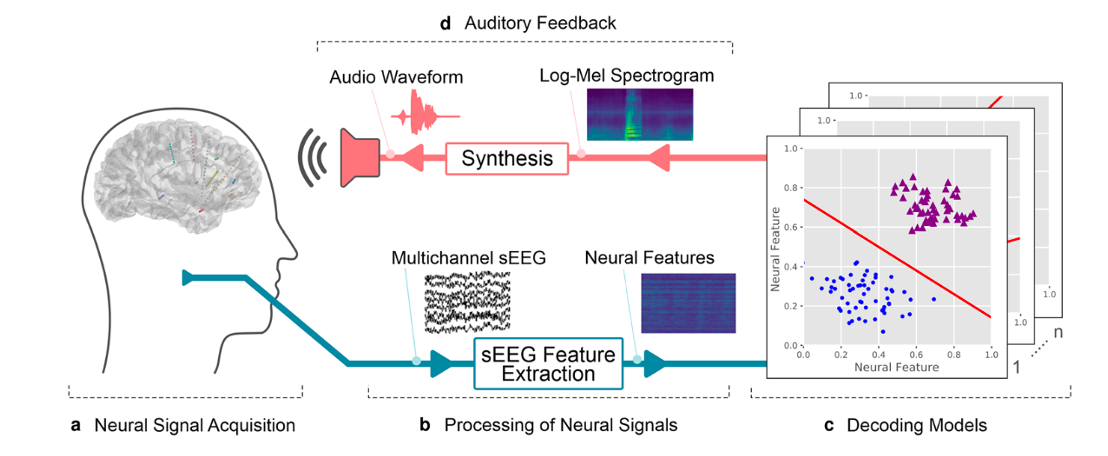
\includegraphics[width=\textwidth]{images/pipelineAngerick.png}
        \caption{Speech synthesis pipeline adapted from Angrick et al.~\cite{Angrick2021}.}
    \end{subfigure}
    \hfill
    \begin{subfigure}[b]{0.47\textwidth}
        \centering
        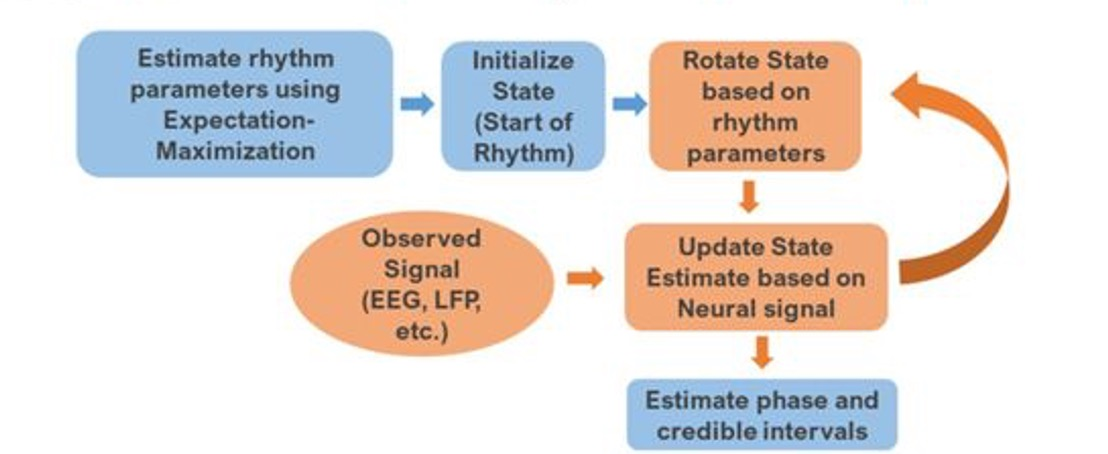
\includegraphics[width=\textwidth]{conceptual_diagram_SSPE}
        \caption{Conceptual SSR feature-extraction pipeline adapted from Wodeyar et al.~\cite{Wodeyar2021}.}
    \end{subfigure}
    \caption{Overview of the decoding workflow and SSR feature extraction. The present analysis replaces conventional fixed-band feature extraction with state-space oscillator tracking while retaining a simple spectrogram decoder for comparison. Credible intervals from the original SSR schematic are not used in the present decoding pipeline.}
    \label{fig:workflow_ssr}
\end{figure}

\section{Methods}

\subsection{Dataset and task}

We used the public intracranial EEG speech production dataset from Verwoert et al.~\cite{dataset}, which includes iEEG recordings, audio recordings, stimulus words, and timing offsets. The data were collected from ten epilepsy participants implanted with stereotactic EEG electrodes for clinical monitoring. Electrode placement was determined by clinical need rather than by the present speech-decoding study; participants had between 54 and 127 recording contacts (1103 in total), and participant-level electrode coverage is summarized in appendix~\ref{app:electrode_locations}. Neural data were sampled at 1024\,Hz and audio at 48\,kHz. Each participant viewed a word for two seconds, read it aloud, and then paused for one second. This yielded 100 trials and approximately 300 seconds of recording per participant. Participant approval for data collection and sharing is documented alongside the original dataset.

\subsection{State-space rhythms model}

For each channel, the SSR model represents the observed iEEG signal as a noisy linear combination of latent oscillatory states. For one oscillator $j$, the two-dimensional latent state $x_t^j=[x_{t,1}^j,x_{t,2}^j]^T \in \mathbb{R}^2$ evolves according to
\begin{equation}
    x_t^j = a_j O(\omega_j)x_{t-1}^j + u_t^j, \quad u_t^j \sim \mathcal{N}(0,\sigma_j^2 I_2),
\end{equation}
where $a_j \in (0,1)$ is a damping coefficient, $u_t^j$ is Gaussian process noise with variance $\sigma_j^2$, and $O(\omega_j)$ is the rotation matrix for central angular frequency $\omega_j=2\pi f_j/F_s$:
\begin{equation}
    O(\omega_j)=
    \begin{pmatrix}
    \cos(\omega_j) & -\sin(\omega_j) \\
    \sin(\omega_j) & \cos(\omega_j)
    \end{pmatrix}.
\end{equation}
The observation equation maps the full hidden state vector $X_t=[(x_t^1)^T,\ldots,(x_t^N)^T]^T$ across all oscillators tracked for this channel onto the observed channel measurement $y_t$:
\begin{equation}
    y_t = M X_t + v_t, \quad v_t \sim \mathcal{N}(0,\sigma_R^2),
\end{equation}
where $M=[1,0,1,0,\ldots,1,0]$ sums the real component of each oscillator and $v_t$ denotes measurement noise~\cite{Matsuda2017,Wodeyar2021}. With the state-transition matrix $\Phi=\mathrm{blockdiag}(a_jO(\omega_j))$ and process-noise covariance $Q=\mathrm{blockdiag}(\sigma_j^2I_2)$, a Kalman filter~\cite{Kalman1960} estimates the latent analytic state at each time point from current and past observations only. Oscillator frequencies, damping coefficients and process-noise variances were initialized per channel (section~\ref{sec:parameters}) and kept fixed during feature extraction; the observation-noise variance was fixed at $\sigma_R^2=1\,\mu\mathrm{V}^2$, which is of the same order as the values estimated during initialization ($\approx0.3\,\mu\mathrm{V}^2$ for an example channel) and small compared with the signal variance (of the order of $10^4\,\mu\mathrm{V}^2$). The filter was started two seconds into the recording; this segment lies within the 10\,s initialization period that was excluded from decoding.

\subsection{SSR oscillators as causal quadrature filters}
\label{sec:ssr_filters}

Because the parameters are fixed, the Kalman gain converges within about one second to a steady-state value $K$ that follows from the discrete algebraic Riccati equation~\cite{Anderson1979}. From then on, the state update
\begin{equation}
    X_t = A X_{t-1} + K y_t, \qquad A=(I-KM)\Phi,
\end{equation}
is a causal, linear, time-invariant filter, and the complex state $z_t^j=x_{t,1}^j+i\,x_{t,2}^j$ of oscillator $j$ is the output of a complex-valued (quadrature) filter applied to the channel signal, with frequency response
\begin{equation}
    H_j(e^{i\omega}) = c_j^{T}\left(I - A e^{-i\omega}\right)^{-1}K,
\end{equation}
where $c_j$ selects $x_{t,1}^j+i\,x_{t,2}^j$ from $X_t$. The amplitude and phase features of an SSR oscillator are therefore the envelope and phase of the signal passed through a narrow-band, causal filter that is centred on the oscillator frequency and whose bandwidth depends jointly on the parameters of all oscillators of the channel. We used this representation to compute, for every oscillator, the $-3$\,dB passband and the group delay $\tau_j=-\mathrm{d}\arg H_j/\mathrm{d}\omega$ at the peak of the response, and compared them with the filters used for the bandpass features (section~\ref{sec:bandpass}). We verified that the steady-state filter reproduces the time-varying Kalman filter used for feature extraction (maximum relative difference in oscillator amplitude $<10^{-8}$ after the first second). It is also considerably cheaper to run, because the update reduces to a set of first-order complex recursions.

\subsection{SSR feature extraction}

Before SSR filtering, each channel was linearly detrended and line noise was attenuated with zero-phase fourth-order band-stop filters ($\pm1$\,Hz) at all harmonics of 50\,Hz from 50 to 450\,Hz; the same preprocessing preceded parameter initialization (section~\ref{sec:parameters}). From the latent state of oscillator $j$, instantaneous amplitude and phase were computed as
\begin{align}
    A_{j,t} &= \sqrt{(x_{t,1}^j)^2+(x_{t,2}^j)^2}, \\
    \Phi_{j,t} &= \operatorname{atan2}(x_{t,2}^j,x_{t,1}^j).
\end{align}
Although SSR provides these quantities at every sample, they were summarized in overlapping 50\,ms windows with a 10\,ms step so that the SSR features could be used with exactly the same windowing, temporal context and decoder as the bandpass features. Three SSR feature sets were evaluated: amplitude only, amplitude plus low-frequency phase, and amplitude plus low-frequency phase plus PAC. Phase and PAC features were extracted only from oscillators below 20\,Hz. For each low-frequency oscillator, PAC was calculated using the amplitude of the first identified high-gamma oscillator within the same channel.

For each window $W$, the amplitude feature was the mean oscillator amplitude:
\begin{equation}
    f_{\mathrm{amp}}(W,j)=\frac{1}{|W|}\sum_{t\in W} A_{j,t}.
\end{equation}
Because phase is circular, phase was represented by the sine and cosine components of the complex phase mean:
\begin{align}
    f_{\sin}(W,j) &= \operatorname{Im}\left(\frac{1}{|W|}\sum_{t\in W} e^{i\Phi_{j,t}}\right), \\
    f_{\cos}(W,j) &= \operatorname{Re}\left(\frac{1}{|W|}\sum_{t\in W} e^{i\Phi_{j,t}}\right).
\end{align}
Within-channel PAC features were defined as the mean vector length of high-gamma amplitude weighted by low-frequency phase~\cite{Canolty2006}:
\begin{equation}
    f_{\mathrm{pac}}(W,j)=\left|\frac{1}{|W|}\sum_{t\in W} A_{\mathrm{HG},t} e^{i\Phi_{j,t}}\right|.
\end{equation}
Note that a 50\,ms window covers only a fraction of a cycle of a slow rhythm, so this quantity is not a PAC estimate in the usual sense, which requires many cycles~\cite{Tort2010,Aru2015}. Within one window the low-frequency phase is nearly constant, so $f_{\mathrm{pac}}$ is close to the window-mean high-gamma amplitude, scaled by the phase concentration within the window (see section~\ref{sec:res_pac}). As a variant that retains the phase at which high-gamma amplitude occurs, we also computed the real and imaginary parts of the same complex mean (phase-resolved PAC, two features per low-frequency oscillator); these are amplitude-phase interaction terms that a linear decoder cannot form from separate amplitude and phase features.

\subsection{Bandpass features}
\label{sec:bandpass}

Bandpass features followed the Verwoert et al. framework~\cite{dataset} and were computed in two ways. As the \emph{offline reference}, we used the original implementation: each channel was linearly detrended, filtered between 70 and 170\,Hz with a fourth-order Butterworth IIR filter applied forward and backward over the whole recording, line-noise harmonics at 100 and 150\,Hz were attenuated with zero-phase band-stop filters, the envelope was obtained with the Hilbert transform of the whole recording, and it was averaged in the same 50\,ms windows as the SSR features. This pipeline has no delay but uses future samples and is therefore not causal. As the \emph{causal baseline}, the same filters were applied forward and backward to the 400\,ms of data ending at the last sample of each 50\,ms window, the Hilbert transform was computed within that buffer, and the envelope was averaged over the final 50\,ms of the buffer. This buffer-wise estimate uses no future data and has no nominal delay, at the cost of estimating the envelope at the edge of the buffer. (Real-time systems of the same group instead filter causally with a continuous filter state and use past-only context~\cite{Angrick2021}; in a pilot participant both causal variants gave equivalent high-gamma decoding.) For the HG + LP models, a fourth-order Butterworth low-pass filter at 20\,Hz was applied in the same way, and the Hilbert amplitude and the sine and cosine of the Hilbert phase of the low-passed signal were added.

To make the two frameworks directly comparable, every SSR feature set has a bandpass counterpart that differs from it in one respect (table~\ref{tab:ladder}): (i) HG + LP amplitude (no phase), mirroring amplitude-only SSR, which also contains low-frequency oscillator amplitudes; (ii) HG + LP (amplitude and phase), mirroring amplitude + phase SSR; (iii) HG + LP + PAC, in which bandpass PAC was computed exactly as the SSR PAC feature from the low-pass Hilbert phase and the high-gamma envelope; and (iv) a \emph{matched bandpass} feature set in which every SSR oscillator of every channel was replaced by a fourth-order Butterworth bandpass filter spanning the $-3$\,dB passband of that oscillator's SSR filter (section~\ref{sec:ssr_filters}), applied buffer-wise as above. The matched bandpass features use the same frequencies, bandwidths, preprocessing, windowing and feature definitions as the SSR features, so that they differ only in how the analytic signal of each oscillator is estimated. A phase-resolved PAC variant was computed for both frameworks.

\begin{table}[!htb]
\centering
\small
\caption{Comparison design. Each row isolates one factor; in the causal analysis all feature sets use past-only temporal context. Results are given in table~\ref{tab:main_results}, figure~\ref{fig:main_results} and table~\ref{tab:contrasts}.}
\label{tab:ladder}
\begin{tabular}{p{0.25\textwidth}p{0.2\textwidth}p{0.44\textwidth}}
\toprule
\textbf{Factor} & \textbf{SSR feature set} & \textbf{Bandpass counterpart(s)} \\
\midrule
Amplitude & Amplitude SSR & HG; HG + LP amplitude; matched bandpass amplitude \\
+ low-frequency phase & Amplitude + phase SSR & HG + LP; matched bandpass amplitude + phase \\
+ PAC & Full SSR & HG + LP + PAC; matched bandpass with PAC \\
Phase-resolved PAC & Full SSR (complex PAC) & HG + LP + complex PAC \\
Estimator (frequencies fixed) & all SSR sets & matched bandpass \\
Causality & causal (all) & buffer-wise (causal) versus whole-recording (offline) bandpass \\
Temporal context & all SSR sets & offline bandpass; past-only versus $\pm200$\,ms \\
\bottomrule
\end{tabular}
\end{table}

\subsection{Parameter initialization with SOMATA}
\label{sec:parameters}

Oscillator frequencies, damping coefficients, and process variances were initialized separately for each subject and channel using the SOMATA iterative state-space fitting procedure~\cite{Beck2022SOMATA} applied to the first 10\,s of each recording after detrending and line-noise removal. SOMATA fits the strongest oscillatory component, uses residual structure to initialize additional components, and refits the full model at each iteration. Model selection used changes in log-likelihood to identify a knee point at which additional oscillators gave diminishing returns. To avoid under-specified channel models, a minimum of three oscillators per channel was enforced.

Because speech decoding is known to depend strongly on high-gamma activity, the initialization pipeline also required at least one high-gamma oscillator (70--170\,Hz) per channel. If the selected SOMATA model did not contain a high-gamma oscillator, higher-iteration models were searched. If no high-gamma oscillator was found within seven iterations, a participant-level high-gamma frequency template was derived from the other channels by applying Gaussian kernel density estimation to identified high-gamma frequencies and selecting the two dominant peaks with \texttt{find\_peaks}. Template oscillator damping and process-noise parameters were estimated by averaging matching oscillators from other channels within a $\pm 7$\,Hz window. Oscillators whose frequency lay within 2\,Hz of a line-noise harmonic (residual line noise after notching) were removed before building the SSR models. The high-gamma fallback was needed for 227 of 1103 channels (20.6\%), ranging from 4 of 60 channels in sub-05 to 98 of 127 channels in sub-06; in an earlier version of the pipeline without the 100\,Hz notch, 39\% of channels needed it. It is a pragmatic heuristic and is treated as a limitation rather than as a fully optimized model-selection procedure. Across participants, 114 of 5238 SOMATA oscillators lay within 2\,Hz of a line-noise harmonic (43 of them at 100\,Hz) and were removed, so that a few channels were left with two oscillators. The resulting models had 2 to 9 oscillators per channel (median 5; 5578 oscillators in total, including template oscillators; appendix~\ref{app:algorithm}).

\begin{figure}[!htb]
    \centering
    \begin{subfigure}[b]{0.47\textwidth}
        \centering
        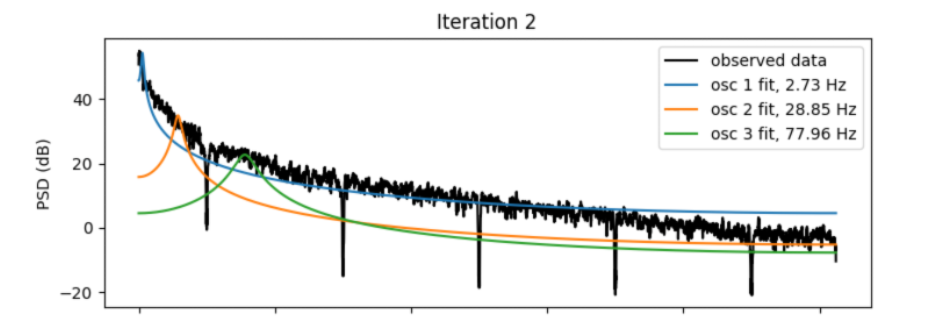
\includegraphics[width=\textwidth]{images/somata_example.png}
        \caption{Iterative SOMATA oscillator fitting.}
    \end{subfigure}
    \hfill
    \begin{subfigure}[b]{0.47\textwidth}
        \centering
        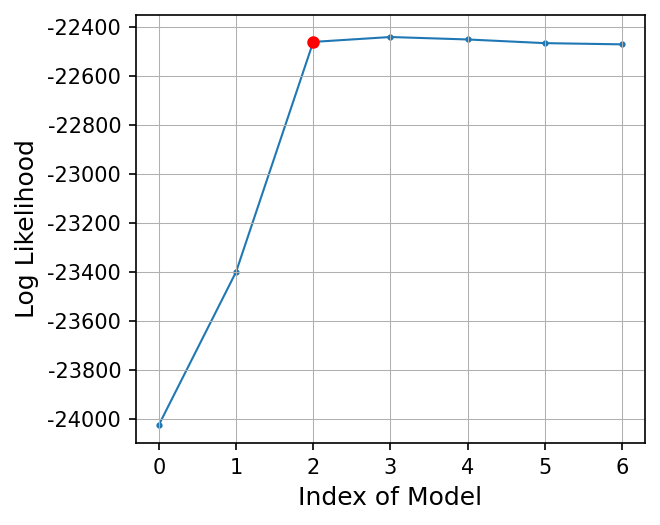
\includegraphics[width=0.48\textwidth]{images/likelihooda.png}
        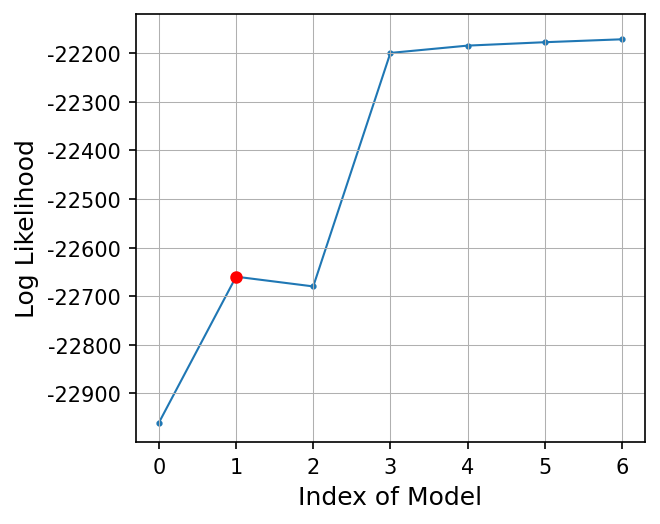
\includegraphics[width=0.48\textwidth]{images/likelihoodb.png}
        \caption{Example log-likelihood knee-point selections.}
    \end{subfigure}
    \caption{Parameter initialization using SOMATA. The log-likelihood criterion identifies the point at which additional oscillators provide diminishing returns, but some channels required minimum-component and high-gamma fallback heuristics.}
    \label{fig:somata_initialization}
\end{figure}

\subsection{Decoder and hyperparameter selection}

We used Partial Least Squares (PLS) regression~\cite{Wold2001} rather than the ordinary linear regression used in the original Verwoert et al. baseline. PLS learns a reduced set of latent components that maximize covariance between neural features and spectrogram coefficients, which is useful when the SSR feature set contains multiple oscillators and feature types. Features from the current window were stacked with those of eight preceding windows at 50\,ms spacing (past-only context, $-400$ to $0$\,ms), so that the decoder uses no future neural data; for comparison with the original framework, we also used the symmetric context of Verwoert et al.~\cite{dataset} (four preceding and four following windows, $\pm200$\,ms), which includes 200\,ms of future data. Features were $z$-scored with the mean and standard deviation of the training folds. The number of PLS components was selected in every outer training set by an inner, contiguous 3-fold cross-validation over 4, 6, 8, 10 and 12 components (nested cross-validation), so that model selection never used test data.

\subsection{Performance evaluation}

Reconstruction performance was evaluated using the Pearson correlation coefficient between the reconstructed spectrogram and the ground-truth speech spectrogram. We followed the non-shuffled 10-fold cross-validation procedure of Verwoert et al.~\cite{dataset}: nine folds were used for training and one fold for testing in each iteration. The first 10 seconds were excluded from decoding evaluation because they were used for SSR parameter initialization. Chance level was estimated as in Verwoert et al.: the ground-truth spectrogram was split at a random point (at least 10\% of the recording from either end), the two parts were swapped, and the correlation with the original spectrogram was computed (1000 repetitions). This null distribution reflects the temporal structure of the speech spectrogram and does not depend on the neural features, so it is the same for all feature sets.

For each participant, validation fold, and Mel-frequency bin, reconstruction correlations were Fisher $r$-to-$z$ transformed and then averaged across the 23 Mel bins, yielding one value per fold. Because all configurations were evaluated on identical cross-validation folds, configurations were compared using paired fold-level differences, averaged within each participant. Group-level inference treated participants as the unit of analysis ($n = 10$): each contrast was tested with a paired $t$-test on participant-mean differences, and we report the mean difference in correlation, $\Delta r$, with its 95\% confidence interval over participants. The planned contrasts were grouped into five families (table~\ref{tab:contrasts}): SSR versus causal bandpass features, SSR versus matched bandpass features, causal versus offline features, temporal context, and phase-resolved PAC. $P$-values were corrected within each family using the Benjamini--Hochberg false discovery rate procedure~\cite{benjamini1995}. Because a non-significant difference does not establish equivalence, we interpret comparable performance through the width of the confidence intervals. Within-participant effects were tested across each participant's $k = 10$ folds with the corrected resampled $t$-test~\cite{nadeau2003}. Within-participant $p$-values were FDR-corrected across participants for each contrast. These statistics are implemented in \texttt{stats\_contrasts.py}.

\subsection{Computational benchmarking and real-time latency analysis}

To evaluate the feasibility of real-time online execution given a $10\text{ ms}$ frame shift, we benchmarked the execution time of the individual components in the SSR feature extraction pipeline. Although feature extraction was performed offline, all SSR algorithms were implemented causally to mirror an online architecture. Rather than re-initializing state structures for every chunk, internal state-space variables were carried forward continuously across adjacent $50\text{ ms}$ blocks, as would be done in a real-time system. Linear detrending and line-noise removal were excluded from the timing evaluation.

The extraction pipeline was segmented into three sequential operations: first, Kalman filtering of each channel per $50\text{ ms}$ block (measured on 20 channels per participant, parallelized over four CPU threads); second, the computation of instantaneous amplitude, phase, and PAC features across all oscillators of all channels for one window; and third, feature stacking across temporal context windows prior to entering the decoder. We additionally timed a streaming implementation of the steady-state filter (section~\ref{sec:ssr_filters}) that updates all channels of a participant sample by sample.

The original timing benchmarks of the per-sample Kalman filter were measured on an Apple M1 with 16~GB memory; the steady-state benchmark ran on a 2.1\,GHz Intel Xeon virtual machine (4 cores, 15~GB memory; Python 3.13, NumPy 2.5).

\section{Results}

\subsection{State-space model validation}

The SSR model was fit across all ten participants and their electrode channels. To assess whether the state-space models captured the intended spectral structure, we compared the raw power spectra with the distribution of tracked oscillator frequencies (figure~\ref{fig:model_fits}). The spectra followed the expected aperiodic $1/f$-like trend~\cite{Donoghue2020}, with high power at low frequencies and lower power at high frequencies. The fitted oscillator distributions included many low-frequency components as well as a distinct high-gamma cluster, most commonly between approximately 70 and 90\,Hz. Part of this cluster consists of template oscillators that were added to channels without a high-gamma component of their own (section~\ref{sec:parameters}), which explains the narrow peaks in participants with many template channels (e.g.\ around 75 and 125\,Hz in sub-06 and above 130\,Hz in sub-09). In sub-05, high-gamma oscillators clustered between 100 and 110\,Hz, close to the 100\,Hz line-noise harmonic, which was not removed in the version of the pipeline used for this figure. Line noise at 100\,Hz was prominent mainly in this participant (more than 3\,dB above neighbouring frequencies in 55 of 60 channels, versus at most 11 channels in any other participant), and the harmonic is now removed before initialization and SSR filtering \todo{regenerate this figure and the SSR results with the corrected notch}.

\begin{figure}[!htb]
    \centering
    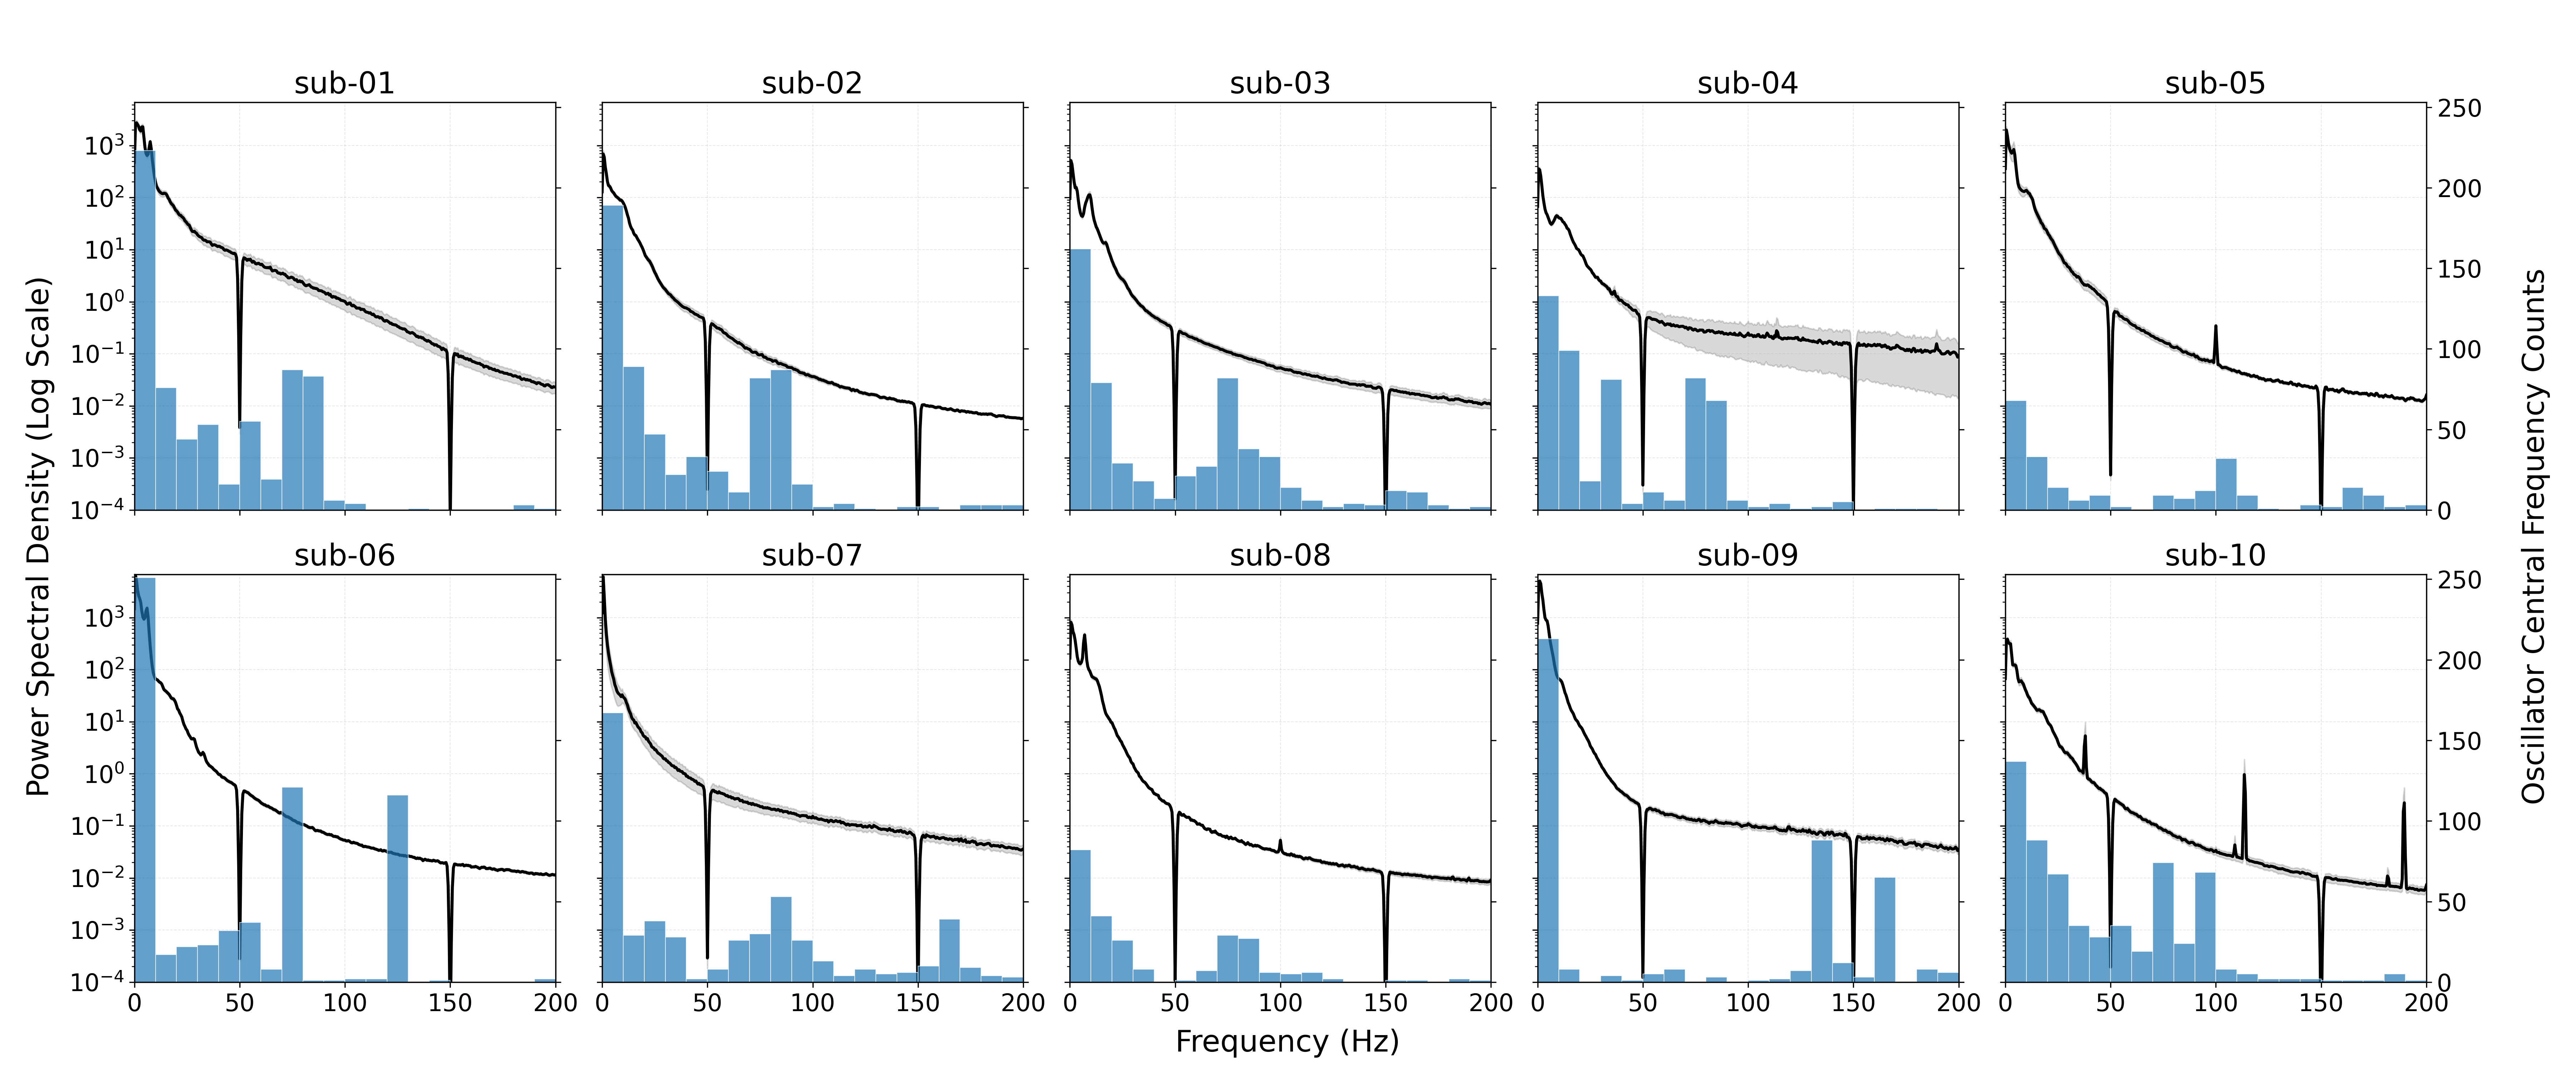
\includegraphics[width=\textwidth]{images/SSR_model_fits_all_subjects.png}
    \caption{Distribution of tracked state-space oscillators versus power spectral density (PSD) across all channels and participants. The left axis shows the average power spectrum (black line; shaded region denotes $\pm$SEM across channels), and the right axis shows the number of tracked oscillator central frequencies in 10 Hz bins, including high-gamma template oscillators. Dips at 50 Hz and 150 Hz reflect line-noise removal; the 100\,Hz harmonic was not removed in this version of the pipeline (visible e.g.\ in sub-05).}
    \label{fig:model_fits}
\end{figure}

\subsection{SSR oscillators are narrow-band causal filters with short delays}
\label{sec:res_filters}

Expressed as filters (section~\ref{sec:ssr_filters}), SSR oscillators had short delays (figure~\ref{fig:filters}). Across all participants, the 1625 high-gamma oscillators had a median $-3$\,dB bandwidth of 56.5\,Hz (interquartile range 30.6--82.0\,Hz) and a median group delay of 6.2\,ms (interquartile range 4.5--11.4\,ms; 95th percentile 18.6\,ms, maximum 28.8\,ms). The 2298 low-frequency oscillators ($<20$\,Hz) had a median bandwidth of 9.3\,Hz and a median group delay of 47.8\,ms (interquartile range 29.1--104.4\,ms); the delay grows as the bandwidth shrinks, and 22 very narrow oscillators below 3\,Hz had delays above 500\,ms. The high-gamma band-pass spans 100\,Hz; applied causally, the fourth-order Butterworth filter delays the pass band by 7.6--19.4\,ms (7.7\,ms at 120\,Hz), comparable to the SSR high-gamma oscillators, whereas the 409-tap FIR filter of the earlier pipeline delayed its output by 199\,ms. SSR oscillators are not steep band-pass filters: far from its own peak, each oscillator state still receives part of the innovation, so that the high-gamma oscillators of sub-01 retained a median of 17\% of their peak gain between 250 and 500\,Hz (1.3\% below 20\,Hz), whereas the Butterworth filter attenuates these frequencies by more than 29\,dB. Because the $1/f$ spectrum puts little power at these frequencies, this leakage is expected to have little effect on the envelopes. The SSR high-gamma amplitude correlated with the high-gamma envelope of the offline (zero-phase) bandpass pipeline with a mean of $r=0.61$ over participants at zero lag (range 0.39--0.80), and the correlation peaked at a lag of 0 or $-10$\,ms (bandpass envelope leading by at most one 10\,ms frame, consistent with the SSR group delay). The buffered causal envelope behaved almost identically (mean $r=0.59$ at zero lag, peak at 0 or $-10$\,ms), whereas the envelope of the causal FIR filter was nearly uncorrelated at zero lag (mean $r=0.11$) and peaked at $+190$ to $+200$\,ms (figure~\ref{fig:filters}C). sub-01, shown in figure~\ref{fig:filters}, had the narrowest high-gamma oscillators (median 21.7\,Hz, group delay 16.6\,ms) and the closest match to the bandpass envelope (peak $r=0.86$).

\begin{figure}[!htb]
    \centering
    \figorplaceholder[width=\textwidth]{images/ssr_vs_bandpass_filters_sub-01.png}
    \caption{SSR oscillators as filters, sub-01. (A) Normalized magnitude response of the SSR oscillators of an example channel, with the zero-phase response $|H|^2$ of the 70--170\,Hz band-pass and 20\,Hz low-pass Butterworth filters of the bandpass features (dashed and dotted). (B) Group delay at the response peak versus oscillator frequency for all oscillators of all channels (colour: $-3$\,dB bandwidth); the dashed line marks the delay of the causal Butterworth band-pass at 120\,Hz (7.7\,ms) and the dotted line the 199\,ms delay of the 409-tap FIR filters of the earlier pipeline. (C) Correlation between SSR high-gamma amplitude features and the high-gamma bandpass envelope as a function of the lag of the bandpass envelope (negative: bandpass leads), for the offline zero-phase pipeline of Verwoert et al., the buffered causal pipeline, and the causal FIR filter of the earlier pipeline (mean $\pm$ SEM over 159 high-gamma oscillators).}
    \label{fig:filters}
\end{figure}

A single-channel example suggested that SSR high-gamma amplitudes can resemble conventional high-gamma bandpass envelopes, whereas low-frequency oscillator amplitudes more closely track slower changes in the raw signal envelope (figure~\ref{fig:ssr_bandpass_validation}A). Across channels, the correlation between bandpass features and SSR high-gamma oscillator amplitudes varied by participant and oscillator (figure~\ref{fig:ssr_bandpass_validation}B). Some high-gamma SSR amplitudes were strongly aligned with the bandpass envelope, with subject-level medians reaching $r=0.765$ and approximately 70\% of high-gamma oscillators exceeding $r=0.70$ in participants 7 and 9. Across all participants, 30.3\% of the high-gamma oscillators exceeded $r=0.70$, and the mean correlation was $r=0.57$. This mixed alignment is expected because a state-space oscillator tracks a narrower, possibly shifted component within the broad high-gamma band. These correlations were computed with a non-causal bandpass filter; with the causal FIR filter used for decoding in an earlier version of this analysis, the unshifted correlation dropped to $r=0.10$ on average because of its 199\,ms delay (figure~\ref{fig:filters}C) \todo{regenerate panel B with the notched SOMATA models and the offline Verwoert envelope, extractHG(timing='verwoert'), and commit the code}.

\begin{figure}[!htb]
    \centering

    \begin{subfigure}[b]{0.95\textwidth}
        \centering
        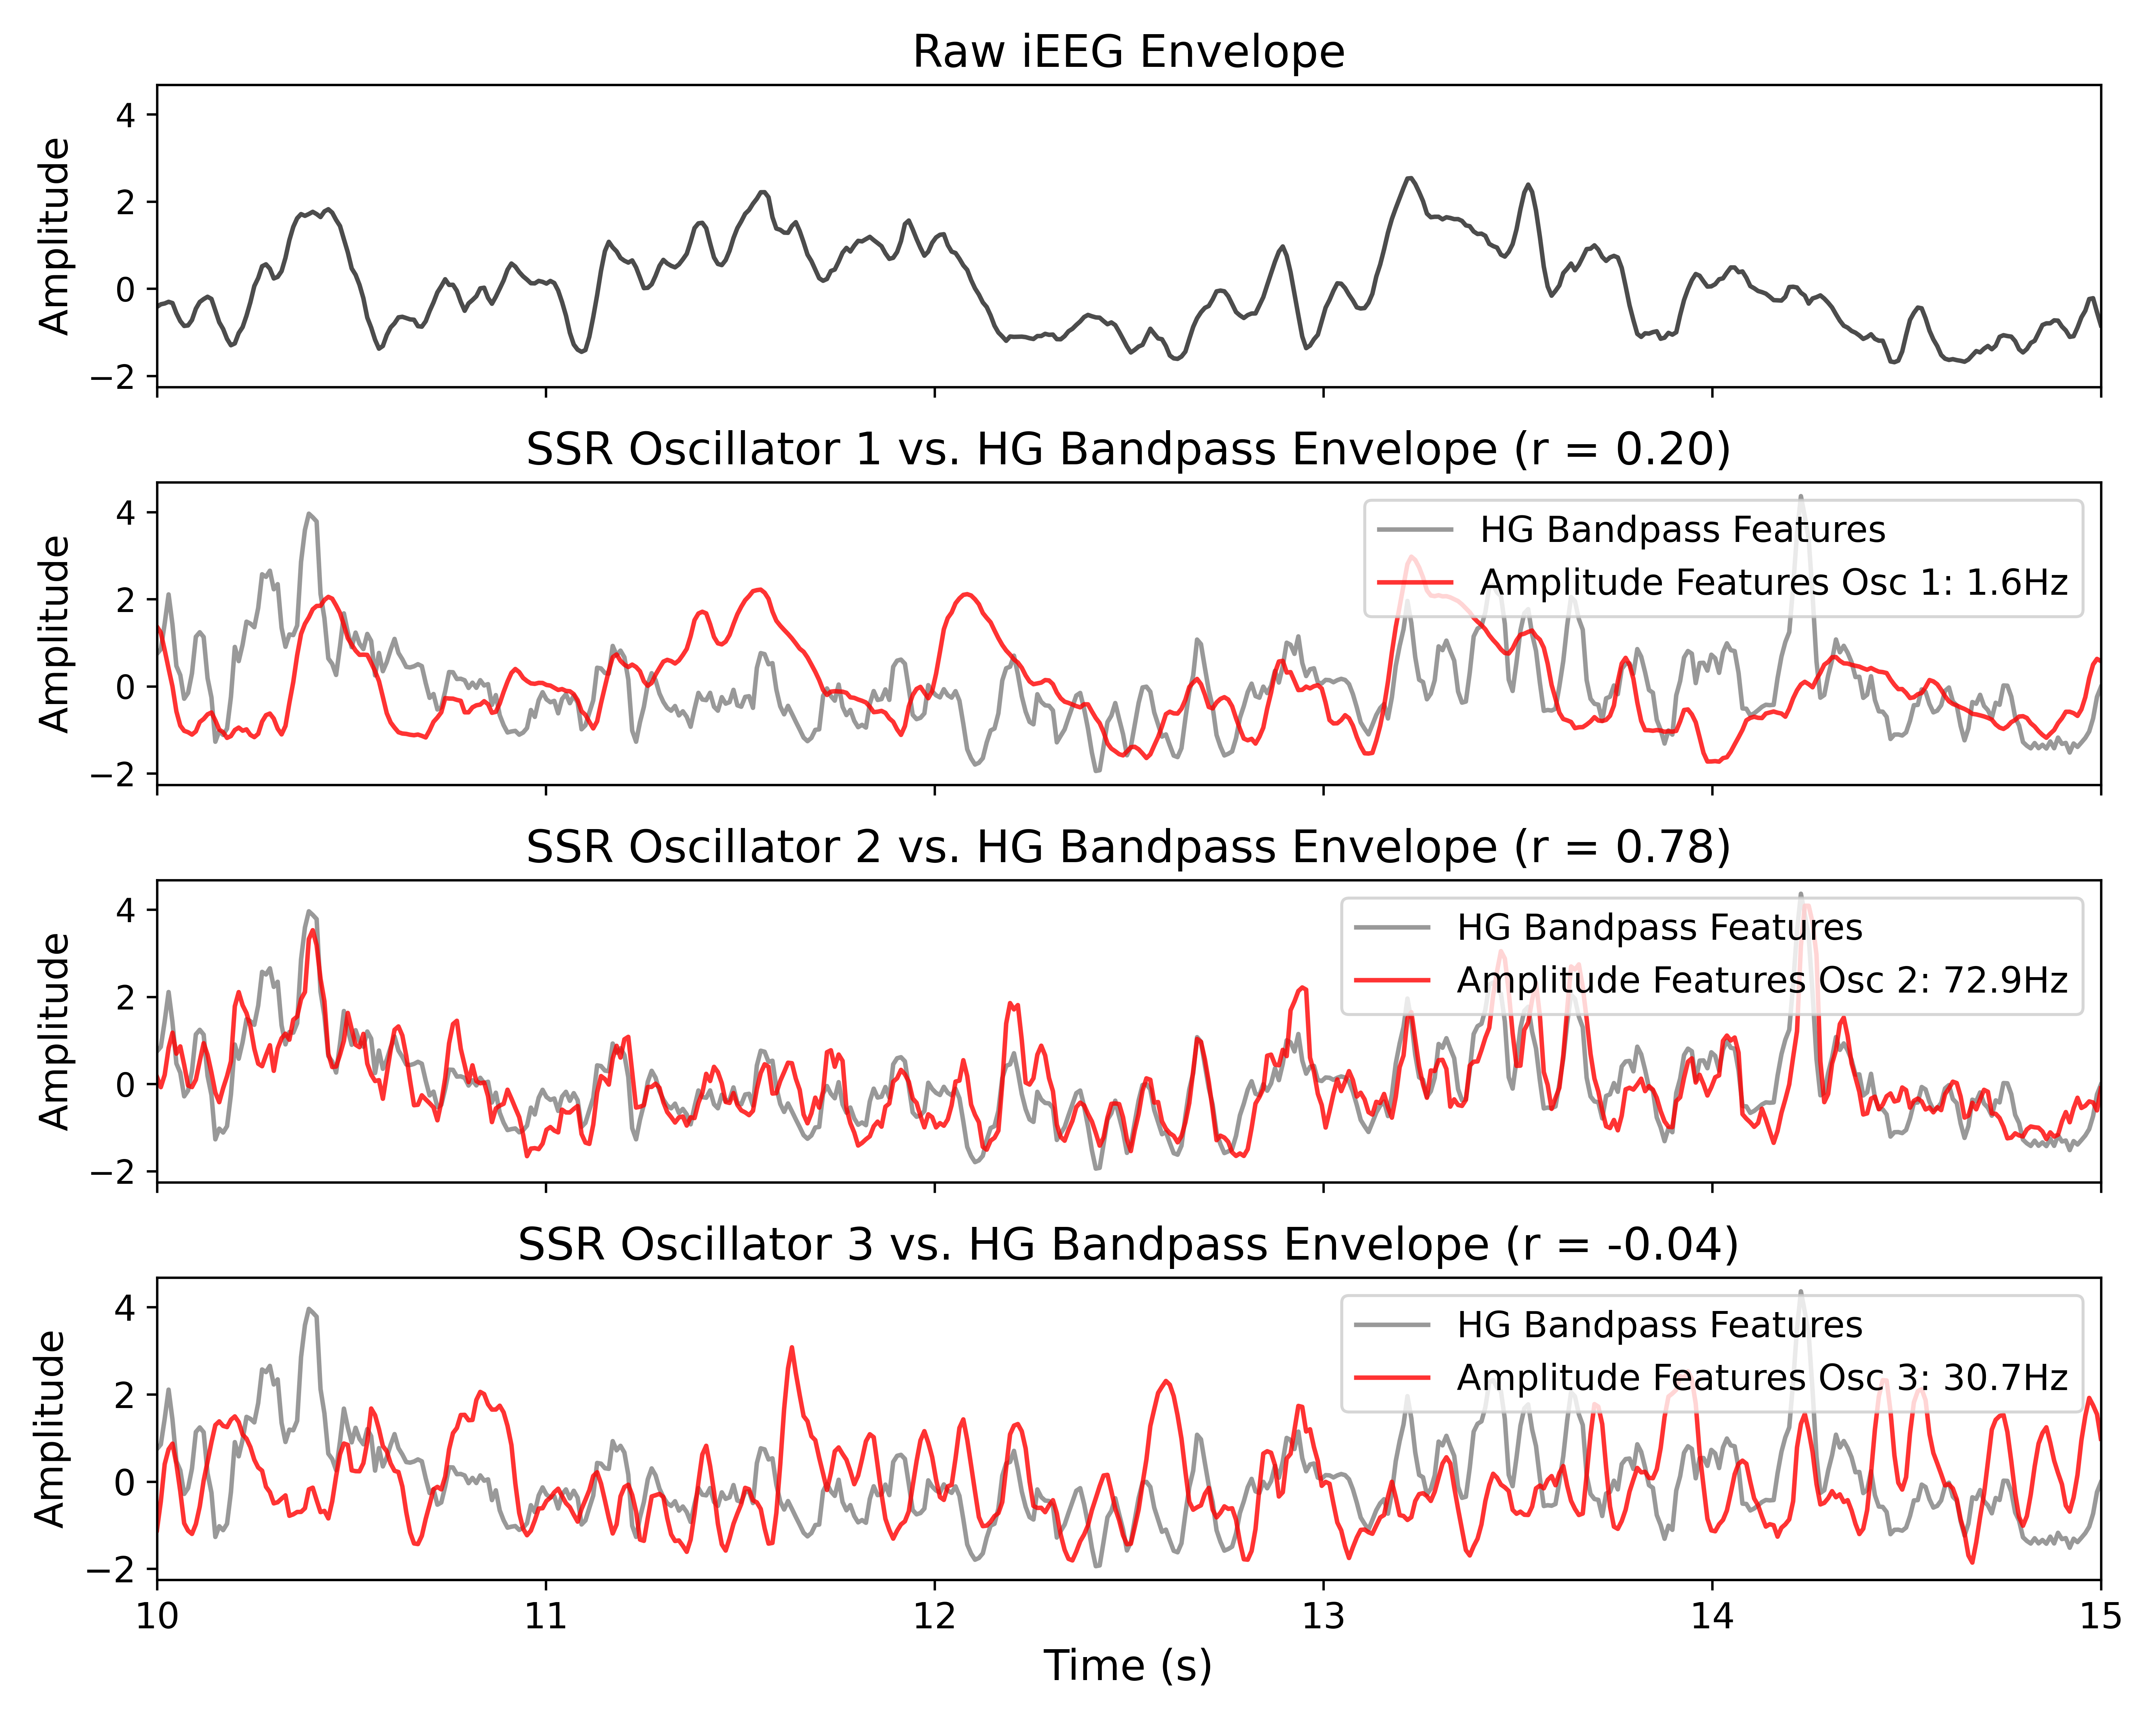
\includegraphics[width=\textwidth]{images/amp_feature_viz.png}
        \caption{Example normalized time-series features.}
    \end{subfigure}

    \vspace{0.75em}

    \begin{subfigure}[b]{0.95\textwidth}
        \centering
        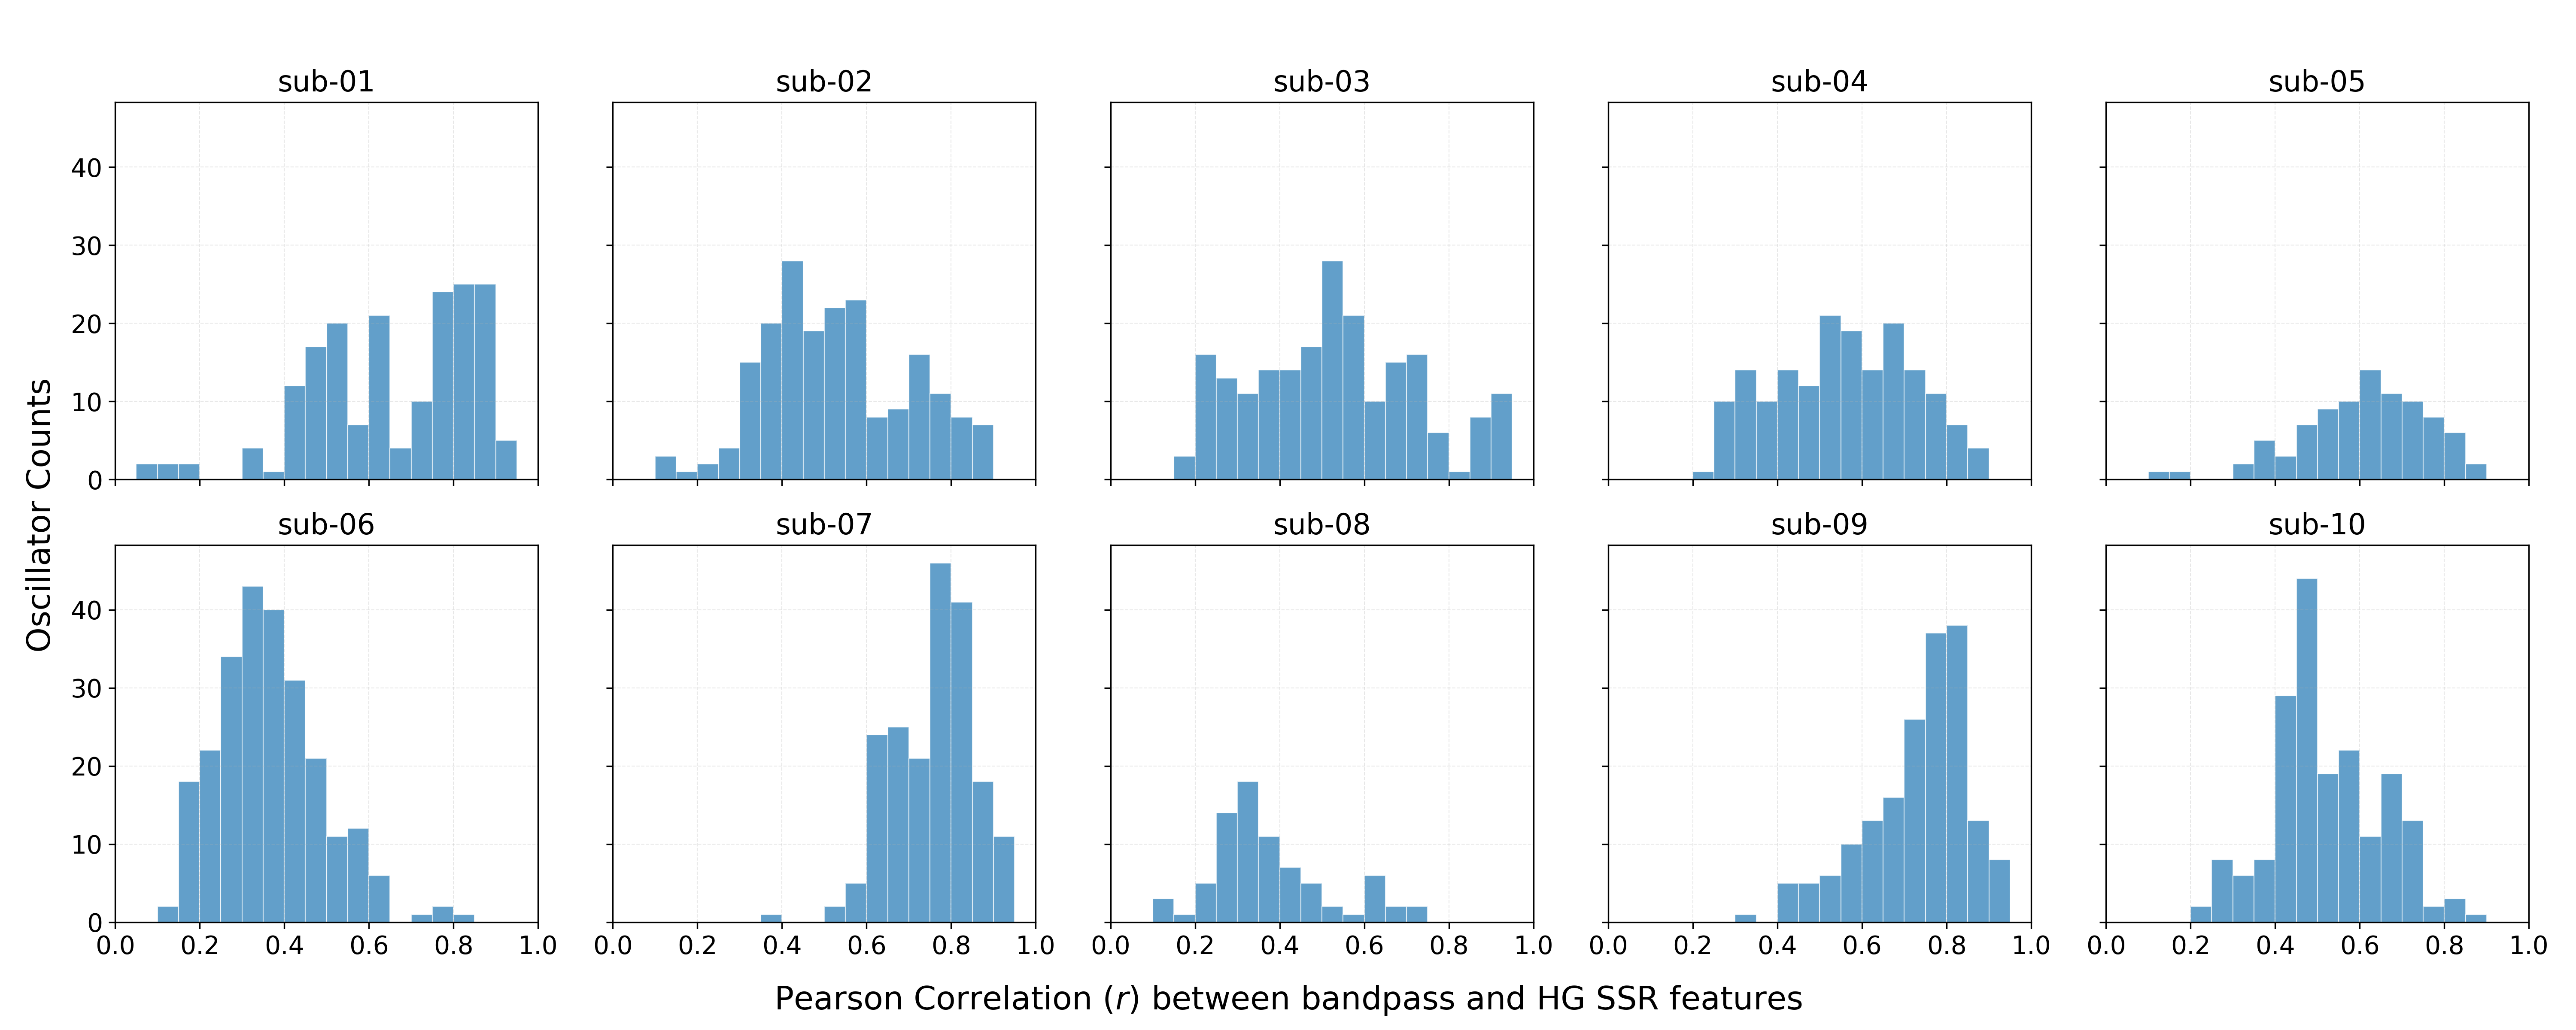
\includegraphics[width=\textwidth]{images/SSR_bandpass_correlation_grid.png}
        \caption{High-gamma SSR amplitude versus bandpass-envelope correlations.}
    \end{subfigure}
    \caption{Validation of SSR features against conventional high-gamma bandpass features. Panel A shows raw iEEG envelope, high-gamma bandpass features, and SSR amplitude features for channel 1 of sub-07. Panel B shows the distribution of Pearson correlations between bandpass features and SSR high-gamma oscillator amplitudes across channels and participants. The HG bandpass features shown in both panels were computed with a non-causal (zero-phase) filter, so that the correlations reflect feature similarity rather than the 199\,ms delay of the causal FIR filter.}
    \label{fig:ssr_bandpass_validation}
\end{figure}


\subsection{Oscillator relevance and PLS weighting}
\label{sec:result_oscImportance}

Correlations between individual SSR amplitude features and the recorded spectrogram suggested that high-gamma oscillators were more speech-informative than non-high-gamma oscillators in most participants (figure~\ref{fig:oscillator_pls}). High-gamma oscillators had higher absolute feature--spectrogram correlations than non-high-gamma oscillators in 9 of 10 participants (one-sided Mann--Whitney test across oscillators, $p<0.001$; oscillators of the same channel are not independent, so these $p$-values are descriptive). Effect sizes varied across participants: several participants showed large shifts ($d>1.0$ for sub-07, sub-08, and sub-10), whereas others showed more modest effects ($d<0.5$ for sub-01, sub-03, and sub-06). This variability motivated the use of PLS rather than manual frequency-subset selection, because explicit feature restriction could overfit to subject-specific spectral patterns. \todo{these correlations compare neural window $t$ with audio window $t+200$\,ms (the spectrogram file is aligned to stacked features) and include the initialization segment; recompute aligned or state the lag}

After fitting the PLS decoder, the absolute PLS weights indicated that the decoder assigned larger weights to localized frequency clusters, especially within the 30--170 Hz range (figure~\ref{fig:oscillator_pls}). For example, sub-10 showed a cluster of high weights between approximately 100 and 110 Hz, whereas sub-02, sub-06, and sub-07 showed flatter weight distributions. These patterns are consistent with the view that speech-relevant information is often concentrated in high-gamma or adjacent frequency ranges, but the precise informative bands vary across participants, likely reflecting both physiology and electrode coverage. Weights of a multivariate decoder reflect both signal and noise suppression and should not be read directly as feature relevance~\cite{Haufe2014}.

\begin{figure}[!htb]
    \centering

    \begin{subfigure}[b]{0.95\textwidth}
        \centering
        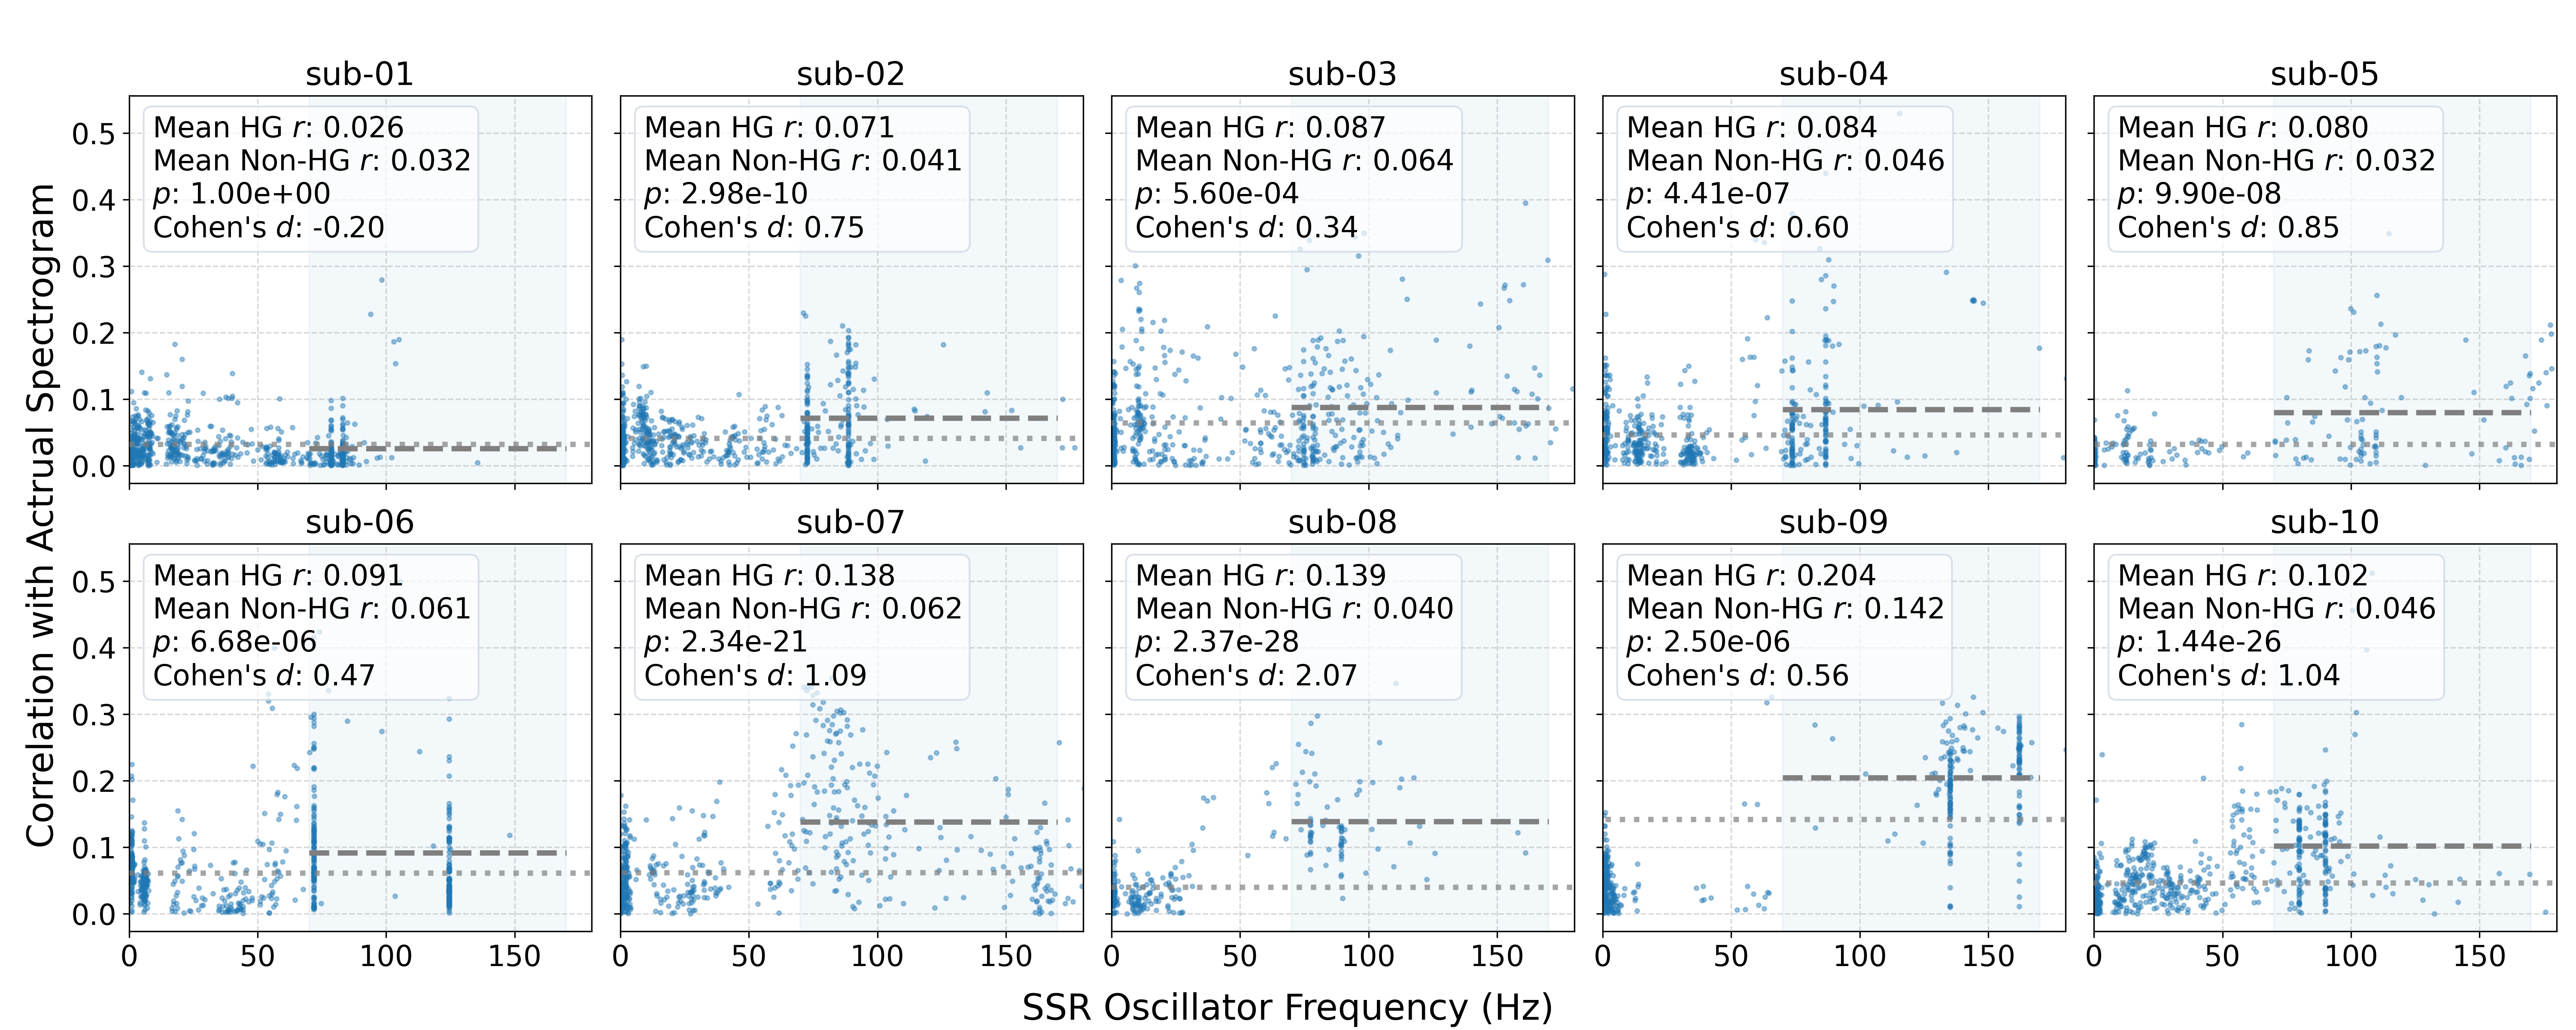
\includegraphics[width=\textwidth]{images/Feature_Audio_Correlations_All_Subjects_new.png}
        \caption{Oscillator amplitude--spectrogram correlations.}
    \end{subfigure}

    \vspace{0.75em}

    \begin{subfigure}[b]{0.95\textwidth}
        \centering
        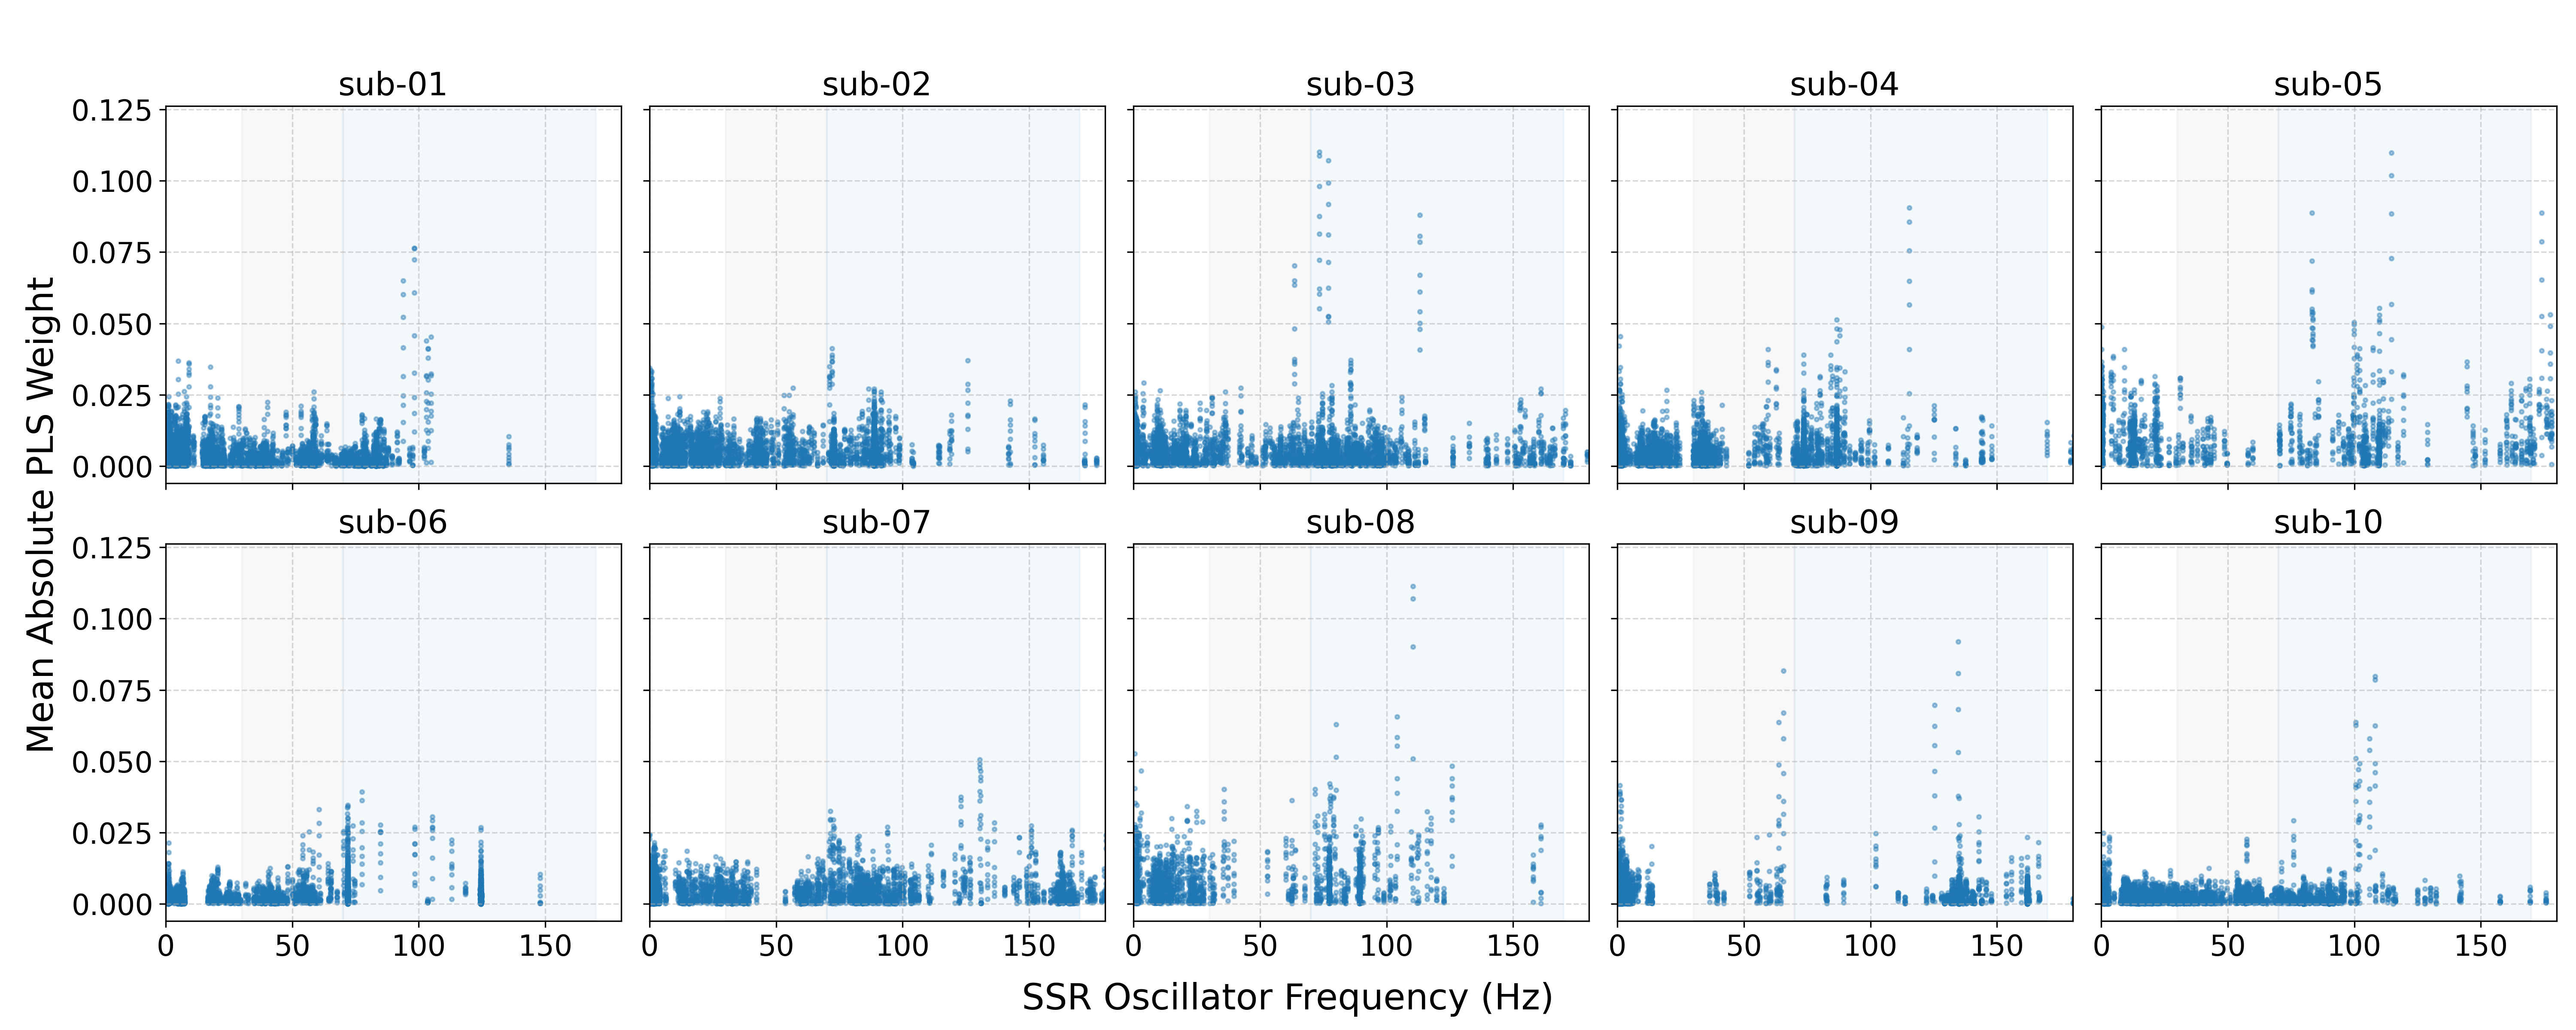
\includegraphics[width=\textwidth]{images/PLS_weights_all_subjects_shaded_new.png}
        \caption{Absolute PLS weights by oscillator frequency.}
    \end{subfigure}

    \caption{Frequency-specific relevance of SSR oscillators. Panel A shows the absolute correlation between individual oscillator amplitude features and the mean of the recorded log-mel spectrogram; high-gamma and non-high-gamma means are indicated by dashed and dotted lines. Panel B shows the absolute PLS weights (averaged over Mel bins and temporal context) assigned to SSR oscillator features in the last cross-validation fold.}
    \label{fig:oscillator_pls}
\end{figure}

\subsection{Decoding performance across feature configurations}
\label{sec:res_decoding}

All feature sets reconstructed the spectrogram far above chance (mean chance correlation $|r|\le0.005$ for every feature set). In the causal pipeline, mean reconstruction correlations ranged from 0.725 to 0.756 (table~\ref{tab:main_results}, figure~\ref{fig:main_results}A), whereas participant means ranged from 0.54 to 0.86, so that differences between participants were an order of magnitude larger than differences between feature sets. All contrasts are listed in table~\ref{tab:contrasts}.

\paragraph{SSR versus causal bandpass features.} In the causal pipeline, SSR features performed on par with bandpass features at every level of the feature hierarchy (figure~\ref{fig:main_results}B). Amplitude-only SSR ($r=0.729$) did not differ from the bandpass model with high-gamma and low-frequency amplitude that it mirrors ($r=0.725$; $\Delta r=+0.003$, 95\% CI $-0.007$ to $0.013$) or from the high-gamma envelope alone ($r=0.736$; $\Delta r=-0.007$, $-0.018$ to $0.004$). With low-frequency phase, SSR ($r=0.753$) matched the HG + LP bandpass model ($r=0.755$; $\Delta r=-0.002$, $-0.010$ to $0.007$), and the full SSR model ($r=0.756$) matched the bandpass model with PAC ($r=0.755$; $\Delta r=+0.001$, $-0.006$ to $0.008$). SSR was better in 3 to 6 of the 10 participants in these comparisons, and no participant showed a significant within-participant difference.

\paragraph{Low-frequency information and PAC.} Low-frequency information improved reconstruction by similar amounts in both frameworks: adding low-frequency phase to the SSR amplitudes increased the correlation by $\Delta r=0.024$ (95\% CI $0.002$ to $0.047$; better in 8 of 10 participants, significantly in 5), and adding low-frequency amplitude and phase to the high-gamma envelope increased it by $\Delta r=0.019$ ($-0.001$ to $0.039$; 8 of 10 participants). Neither gain survived correction within its contrast family ($p=0.021$ and $p=0.040$ uncorrected; $p_{\mathrm{FDR}}=0.16$). Low-frequency amplitude without phase did not help the bandpass features (HG + LP amplitude, $r=0.725$, versus HG, $r=0.736$), so the gain came with the phase features. PAC added little in either framework (SSR: $\Delta r=+0.003$, $-0.003$ to $0.009$; bandpass: $\Delta r=+0.000$, $-0.003$ to $0.003$; section~\ref{sec:res_pac}).

\paragraph{Estimator at matched frequencies.} When every SSR oscillator was replaced by a Butterworth bandpass filter spanning its passband, the two estimators gave practically identical results at all three feature levels ($|\Delta r|\le0.0005$; 95\% CIs within $\pm0.015$ for amplitude and $\pm0.010$ for the sets with phase; 5 of 10 participants favoured SSR in each comparison). In this pipeline, decoding accuracy was therefore determined by which frequencies were tracked rather than by whether their analytic signal was estimated with a Kalman filter or with buffer-wise zero-phase filtering and a Hilbert transform.

\paragraph{Causal versus offline features.} The offline bandpass pipeline of Verwoert et al., which filters and Hilbert-transforms the whole recording and therefore uses future samples, gave the highest correlations (HG, $r=0.740$; HG + LP, $r=0.763$; HG + LP + PAC, $r=0.764$). The causal buffered bandpass features were consistently below their offline counterparts (HG: $\Delta r=-0.004$, $-0.007$ to $-0.001$; HG + LP: $\Delta r=-0.008$, $-0.013$ to $-0.003$; both $p_{\mathrm{FDR}}=0.012$, lower in 9 of 10 participants), and the causal SSR features were below the offline features by similar margins ($\Delta r=-0.011$ to $-0.008$; $p_{\mathrm{FDR}}=0.055$--$0.12$; lower in 7 to 9 participants). This loss is the cost of estimating features causally, and it was the same for both causal frameworks.

\paragraph{Temporal context.} Replacing the past-only context ($-400$ to $0$\,ms) with the symmetric context of the original framework ($\pm200$\,ms), which adds 200\,ms of future neural data, did not change performance consistently (all $p_{\mathrm{FDR}}\ge0.29$; figure~\ref{fig:main_results}C). For the feature sets with low-frequency phase, the symmetric context gave slightly higher correlations (SSR amplitude + phase: past-only $\Delta r=-0.012$, $-0.024$ to $0.001$; offline HG + LP: $\Delta r=-0.010$, $-0.025$ to $0.005$), whereas for the high-gamma envelope alone the past-only context was better in 6 of 10 participants ($\Delta r=+0.022$, $-0.008$ to $0.051$). With the symmetric context, the SSR models reached $r=0.765$ (amplitude + phase and full model) and the offline HG + LP bandpass model $r=0.773$.

\paragraph{Model selection.} Nested cross-validation selected a median of 4 to 10 PLS components, depending on the feature set (table~\ref{tab:main_results}). Across all feature sets and outer folds, the smallest value of the grid (4) was chosen in 13.6\% and the largest (12) in 7.3\% of cases; the high-gamma-only feature sets chose 4 components in half of the folds.

Performance across consecutive validation folds is shown in appendix~\ref{app:tempstability}. Performance remained stable, indicating that the initialized oscillator parameters remained useful throughout the recordings, although longer recordings and online validation would be needed to assess parameter drift more rigorously \todo{the stability figure is from the earlier version of the analysis; regenerate with the causal results}.

\begin{figure}[!htb]
    \centering
    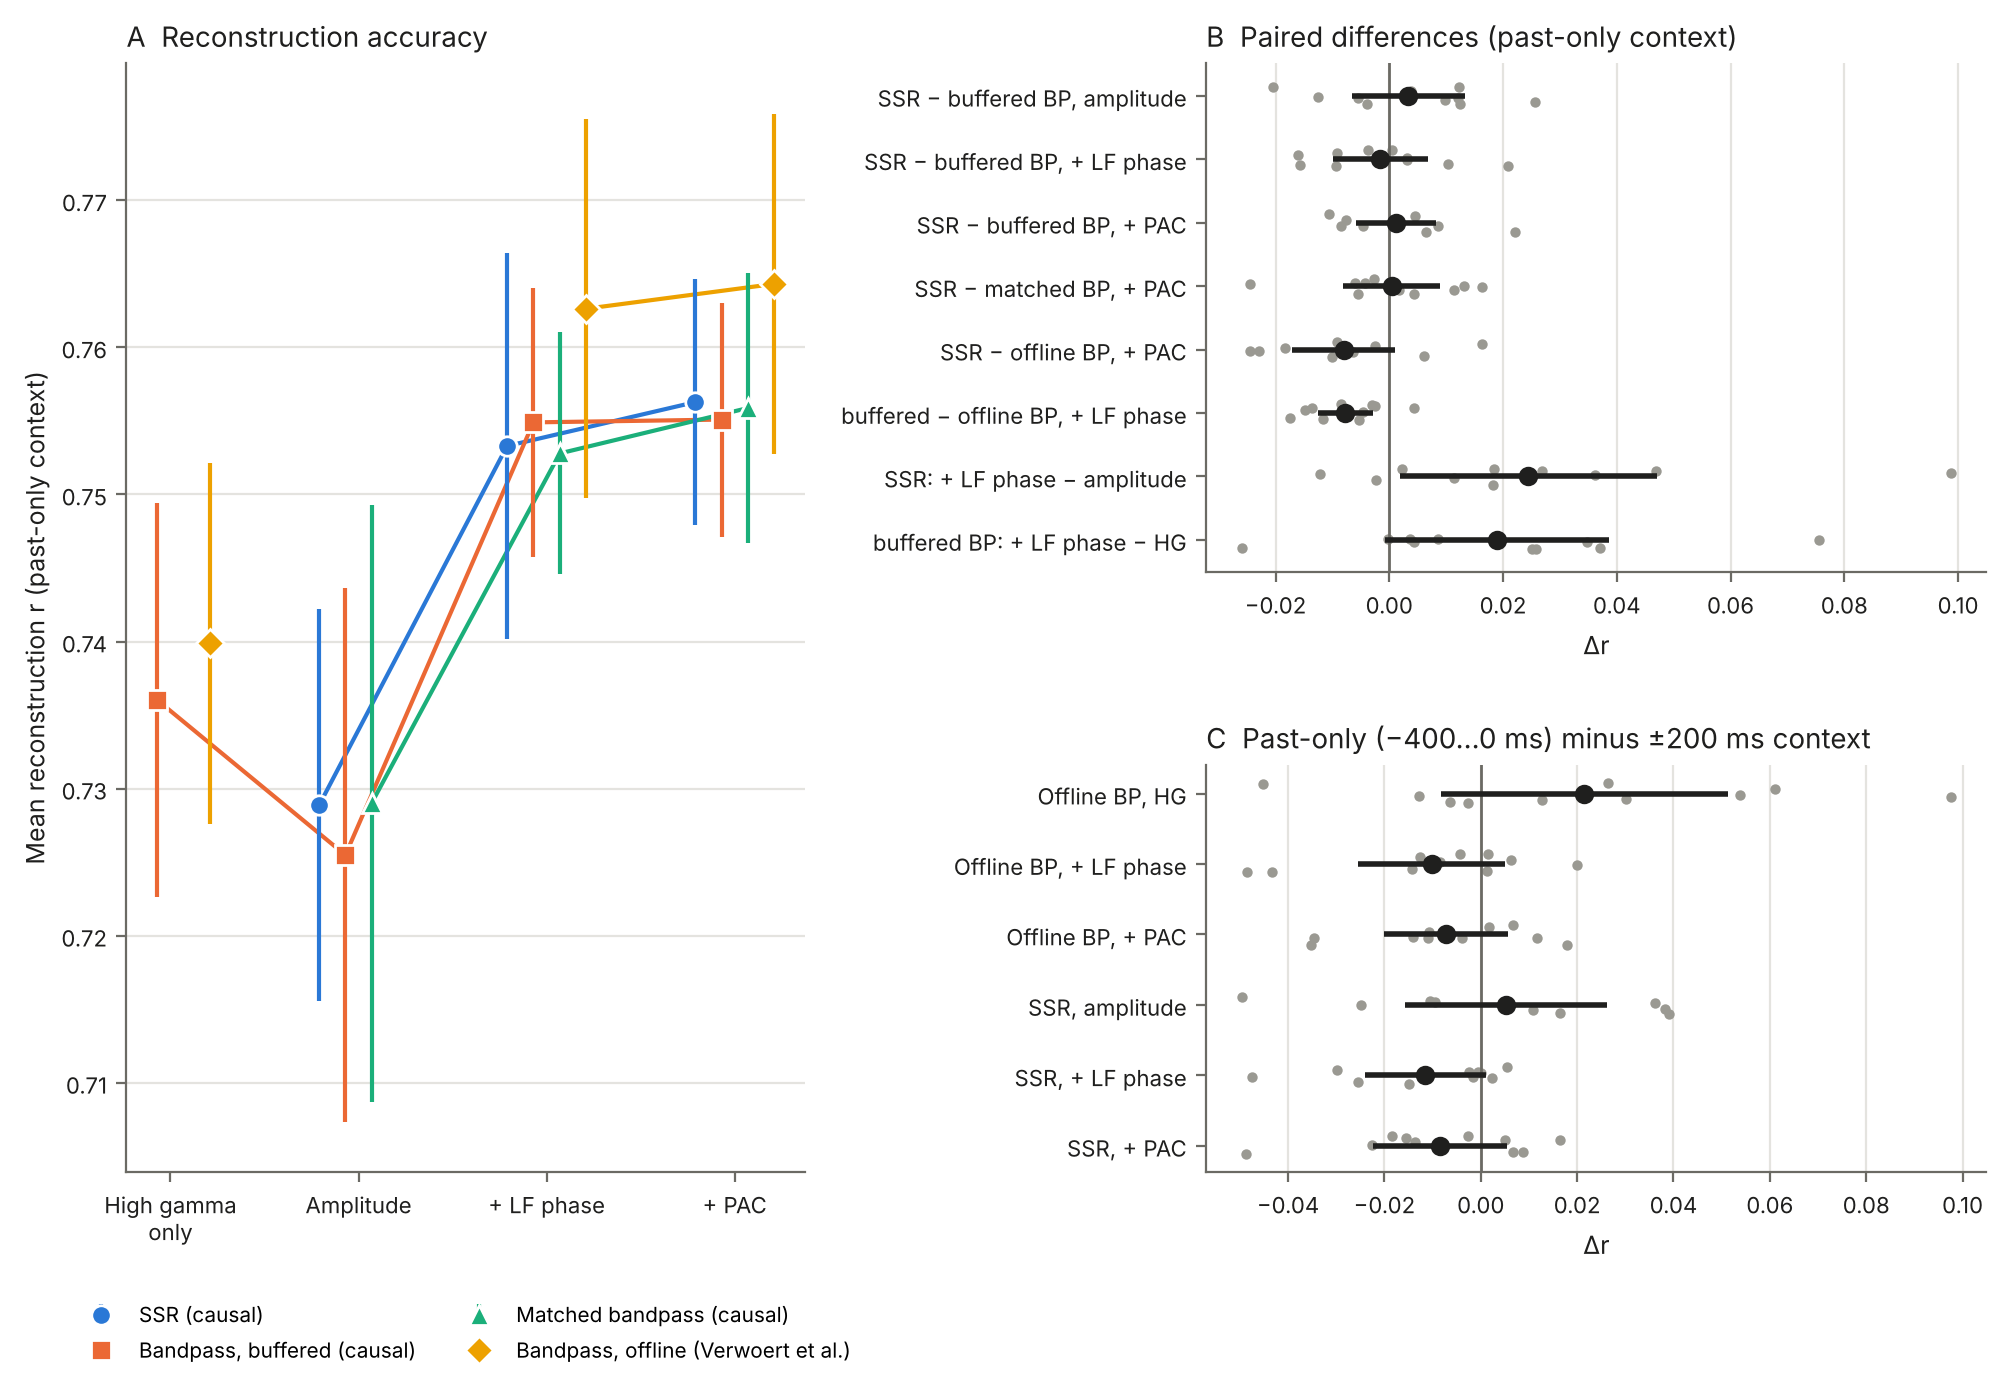
\includegraphics[width=\linewidth]{images/main_results.png}
    \caption{Reconstruction accuracy of SSR and bandpass features ($n=10$ participants). (A) Mean reconstruction correlation with past-only temporal context for each framework and feature level; error bars are 95\% within-participant confidence intervals (Cousineau--Morey). Bandpass amplitude: high-gamma envelope plus low-pass amplitude; matched bandpass: Butterworth filters at the passbands of the SSR oscillators; offline bandpass: whole-recording zero-phase filtering and Hilbert transform as in Verwoert et al.~\cite{dataset}. (B) Paired differences in reconstruction correlation; grey dots are participants, black markers the mean and 95\% confidence interval. (C) Past-only minus symmetric ($\pm200$\,ms) temporal context. BP, bandpass; LF, low-frequency ($<20$\,Hz).}
    \label{fig:main_results}
\end{figure}

\begin{table}[!htb]
\centering
\small
\caption{Reconstruction correlations (mean $\pm$ SD over participants; mean over folds and Mel bins per participant) for past-only ($-400$ to $0$\,ms) and symmetric ($\pm200$\,ms) temporal context, and the median number of PLS components selected by nested cross-validation (past-only context). Causal bandpass features were computed on a 400\,ms buffer of past data; offline bandpass features as in Verwoert et al.~\cite{dataset}. Mean chance correlations were $|r|\le0.005$ for all feature sets.}
\label{tab:main_results}
% generated by summarize_main.py
\begin{tabular}{lccc}
\toprule
\textbf{Feature set} & \textbf{Past-only} & \textbf{$\pm200$\,ms} & \textbf{PLS comp.} \\
\midrule
\multicolumn{4}{l}{\textit{Causal bandpass (buffered)}} \\
\quad HG & $0.736 \pm 0.078$ & -- & 5 \\
\quad HG + LP amplitude & $0.725 \pm 0.088$ & -- & 6 \\
\quad HG + LP (amplitude + phase) & $0.755 \pm 0.063$ & -- & 8 \\
\quad HG + LP + PAC & $0.755 \pm 0.063$ & -- & 8 \\
\quad HG + LP + phase-resolved PAC & $0.755 \pm 0.063$ & -- & 10 \\
\quad HG + LP amplitude + LMP (post hoc) & $0.762 \pm 0.060$ & -- & -- \\
\multicolumn{4}{l}{\textit{Matched bandpass (buffered)}} \\
\quad Amplitude & $0.729 \pm 0.091$ & -- & 6 \\
\quad Amplitude + phase & $0.753 \pm 0.068$ & -- & 8 \\
\quad Amplitude + phase + PAC & $0.756 \pm 0.068$ & -- & 6 \\
\multicolumn{4}{l}{\textit{SSR (causal)}} \\
\quad Amplitude & $0.729 \pm 0.082$ & $0.724 \pm 0.095$ & 6 \\
\quad Amplitude + phase & $0.753 \pm 0.062$ & $0.765 \pm 0.068$ & 6 \\
\quad Amplitude + phase + PAC & $0.756 \pm 0.062$ & $0.765 \pm 0.069$ & 6 \\
\quad Amplitude + phase + phase-resolved PAC & $0.752 \pm 0.062$ & -- & 8 \\
\multicolumn{4}{l}{\textit{Offline bandpass (Verwoert et al.)}} \\
\quad HG & $0.740 \pm 0.076$ & $0.718 \pm 0.098$ & 4 \\
\quad HG + LP (amplitude + phase) & $0.763 \pm 0.061$ & $0.773 \pm 0.065$ & 8 \\
\quad HG + LP + PAC & $0.764 \pm 0.062$ & $0.772 \pm 0.065$ & 6 \\
\bottomrule
\end{tabular}

\end{table}

\begin{table}[!htb]
\centering
\scriptsize
\setlength{\tabcolsep}{3pt}
\caption{Planned contrasts (past-only context unless stated). $\Delta r$: mean paired difference in reconstruction correlation over participants with its 95\% confidence interval; $t(9)$ and $p$ from paired $t$-tests on Fisher-$z$ differences, with Benjamini--Hochberg correction within each family; last column: participants in which the first configuration was better. BP, bandpass; HG, high gamma; LP, low pass ($<20$\,Hz).}
\label{tab:contrasts}
\resizebox{\textwidth}{!}{% generated by stats_contrasts.py --preset main
\begin{tabular}{lccccc}
\toprule
\textbf{Contrast} & $\boldsymbol{\Delta r}$ & \textbf{95\% CI} & $\boldsymbol{t(9)}$ & $\boldsymbol{p}$ / $\boldsymbol{p_{\mathrm{FDR}}}$ & \textbf{Better} \\
\midrule
\multicolumn{6}{l}{\textit{A. causal pipeline (past-only context): SSR vs buffered bandpass}} \\
\quad BP: HG + LP $-$ BP: HG & $+0.019$ & $[-0.001, +0.039]$ & $+2.40$ & 0.040 / 0.161 & 8/10 \\
\quad SSR: amp. $-$ BP: HG & $-0.007$ & $[-0.018, +0.004]$ & $-1.06$ & 0.316 / 0.633 & 3/10 \\
\quad SSR: amp. $-$ BP: HG + LP amp. & $+0.003$ & $[-0.007, +0.013]$ & $+0.69$ & 0.505 / 0.716 & 6/10 \\
\quad SSR: amp. + phase $-$ SSR: amp. & $+0.024$ & $[+0.002, +0.047]$ & $+2.80$ & 0.021 / 0.161 & 8/10 \\
\quad SSR: amp. + phase $-$ BP: HG + LP & $-0.002$ & $[-0.010, +0.007]$ & $-0.64$ & 0.537 / 0.716 & 5/10 \\
\quad SSR: amp. + phase + PAC $-$ SSR: amp. + phase & $+0.003$ & $[-0.003, +0.009]$ & $+1.55$ & 0.154 / 0.412 & 8/10 \\
\quad SSR: amp. + phase + PAC $-$ BP: HG + LP + PAC & $+0.001$ & $[-0.006, +0.008]$ & $+0.32$ & 0.753 / 0.861 & 6/10 \\
\quad BP: HG + LP + PAC $-$ BP: HG + LP & $+0.000$ & $[-0.003, +0.003]$ & $+0.09$ & 0.930 / 0.930 & 5/10 \\
\multicolumn{6}{l}{\textit{B. estimator at matched frequencies (past-only)}} \\
\quad SSR: amp. $-$ matched BP: amp. & $-0.000$ & $[-0.015, +0.015]$ & $-0.27$ & 0.796 / 0.917 & 5/10 \\
\quad SSR: amp. + phase $-$ matched BP: amp. + phase & $+0.001$ & $[-0.009, +0.010]$ & $-0.11$ & 0.917 / 0.917 & 5/10 \\
\quad SSR: amp. + phase + PAC $-$ matched BP: amp. + phase + PAC & $+0.000$ & $[-0.008, +0.009]$ & $-0.13$ & 0.899 / 0.917 & 5/10 \\
\multicolumn{6}{l}{\textit{C. causal SSR vs offline Verwoert bandpass (past-only) and cost of causal bandpass}} \\
\quad SSR: amp. $-$ offline BP: HG & $-0.011$ & $[-0.024, +0.002]$ & $-1.72$ & 0.120 / 0.120 & 3/10 \\
\quad SSR: amp. + phase $-$ offline BP: HG + LP & $-0.009$ & $[-0.018, -0.000]$ & $-2.51$ & 0.033 / 0.055 & 1/10 \\
\quad SSR: amp. + phase + PAC $-$ offline BP: HG + LP + PAC & $-0.008$ & $[-0.017, +0.001]$ & $-2.05$ & 0.070 / 0.088 & 2/10 \\
\quad BP: HG $-$ offline BP: HG & $-0.004$ & $[-0.006, -0.001]$ & $-3.81$ & 0.004 / 0.012 & 1/10 \\
\quad BP: HG + LP $-$ offline BP: HG + LP & $-0.008$ & $[-0.013, -0.003]$ & $-3.73$ & 0.005 / 0.012 & 1/10 \\
\multicolumn{6}{l}{\textit{D. temporal context (past-only minus $\pm$200 ms)}} \\
\quad offline BP: HG $-$ offline BP: HG ($\pm$200\,ms) & $+0.022$ & $[-0.008, +0.051]$ & $+1.27$ & 0.236 / 0.295 & 6/10 \\
\quad offline BP: HG + LP $-$ offline BP: HG + LP ($\pm$200\,ms) & $-0.010$ & $[-0.025, +0.005]$ & $-1.61$ & 0.142 / 0.295 & 4/10 \\
\quad SSR: amp. $-$ SSR: amp. ($\pm$200\,ms) & $+0.005$ & $[-0.016, +0.026]$ & $+0.23$ & 0.822 / 0.822 & 6/10 \\
\quad SSR: amp. + phase $-$ SSR: amp. + phase ($\pm$200\,ms) & $-0.011$ & $[-0.024, +0.001]$ & $-2.08$ & 0.067 / 0.295 & 3/10 \\
\quad SSR: amp. + phase + PAC $-$ SSR: amp. + phase + PAC ($\pm$200\,ms) & $-0.008$ & $[-0.022, +0.005]$ & $-1.44$ & 0.183 / 0.295 & 4/10 \\
\multicolumn{6}{l}{\textit{E. phase-resolved PAC}} \\
\quad SSR: amp. + phase + PAC (phase-resolved) $-$ SSR: amp. + phase + PAC & $-0.004$ & $[-0.010, +0.002]$ & $-2.05$ & 0.071 / 0.141 & 2/10 \\
\quad BP: HG + LP + PAC (phase-resolved) $-$ BP: HG + LP + PAC & $-0.000$ & $[-0.005, +0.004]$ & $-0.26$ & 0.804 / 0.804 & 5/10 \\
\bottomrule
\end{tabular}
}
\end{table}

\subsection{PAC features are dominated by high-gamma amplitude}
\label{sec:res_pac}

Within a 50\,ms window the phase of a slow oscillator changes little, so the PAC feature mostly reproduces the window-mean high-gamma amplitude. Across participants, the PAC features of the 2298 low-frequency oscillators correlated with the amplitude feature of the channel's high-gamma oscillator with a median of $r=0.83$ (participant medians 0.70--0.93; oscillators below 8\,Hz: $r=0.89$). This redundancy explains why the PAC features added little beyond amplitude and phase (section~\ref{sec:res_decoding}). The phase-resolved variant, which keeps the phase at which high-gamma amplitude occurs and thus provides amplitude--phase interaction terms that a linear decoder cannot form itself, did not help either: it changed the correlation by $\Delta r=-0.004$ for SSR ($-0.010$ to $0.002$) and by $\Delta r=-0.000$ for the bandpass features ($-0.005$ to $0.004$; table~\ref{tab:contrasts}, family E). With 50\,ms windows and a linear decoder, cross-frequency features therefore added no information beyond high-gamma amplitude and low-frequency phase.

\subsection{Spectrogram structure}

Example spectrogram reconstructions for sub-01 are shown in figure~\ref{fig:spectrograms}. The ground-truth spectrogram contains clear harmonic structure and temporal gaps, whereas both reconstructions are smoother and have higher overall intensity during silence. \todo{quantify smoothing, e.g.\ reconstruction-to-ground-truth standard deviation ratio, before claiming it differs between models} Absolute error tracks were similar across SSR and bandpass reconstructions, with participant-level correlations between the two error tracks ranging from $r=0.64$ in sub-01 to $r=0.78$ in sub-10 \todo{recompute from the final res\_ predictions; the notebook used earlier prediction files and the previous draft reported 0.54--0.76}. These shared errors suggest that many reconstruction failures reflect stimulus-locked acoustic transitions that are difficult for both feature sets and the linear decoder.

\begin{figure}[!htb]
    \centering
    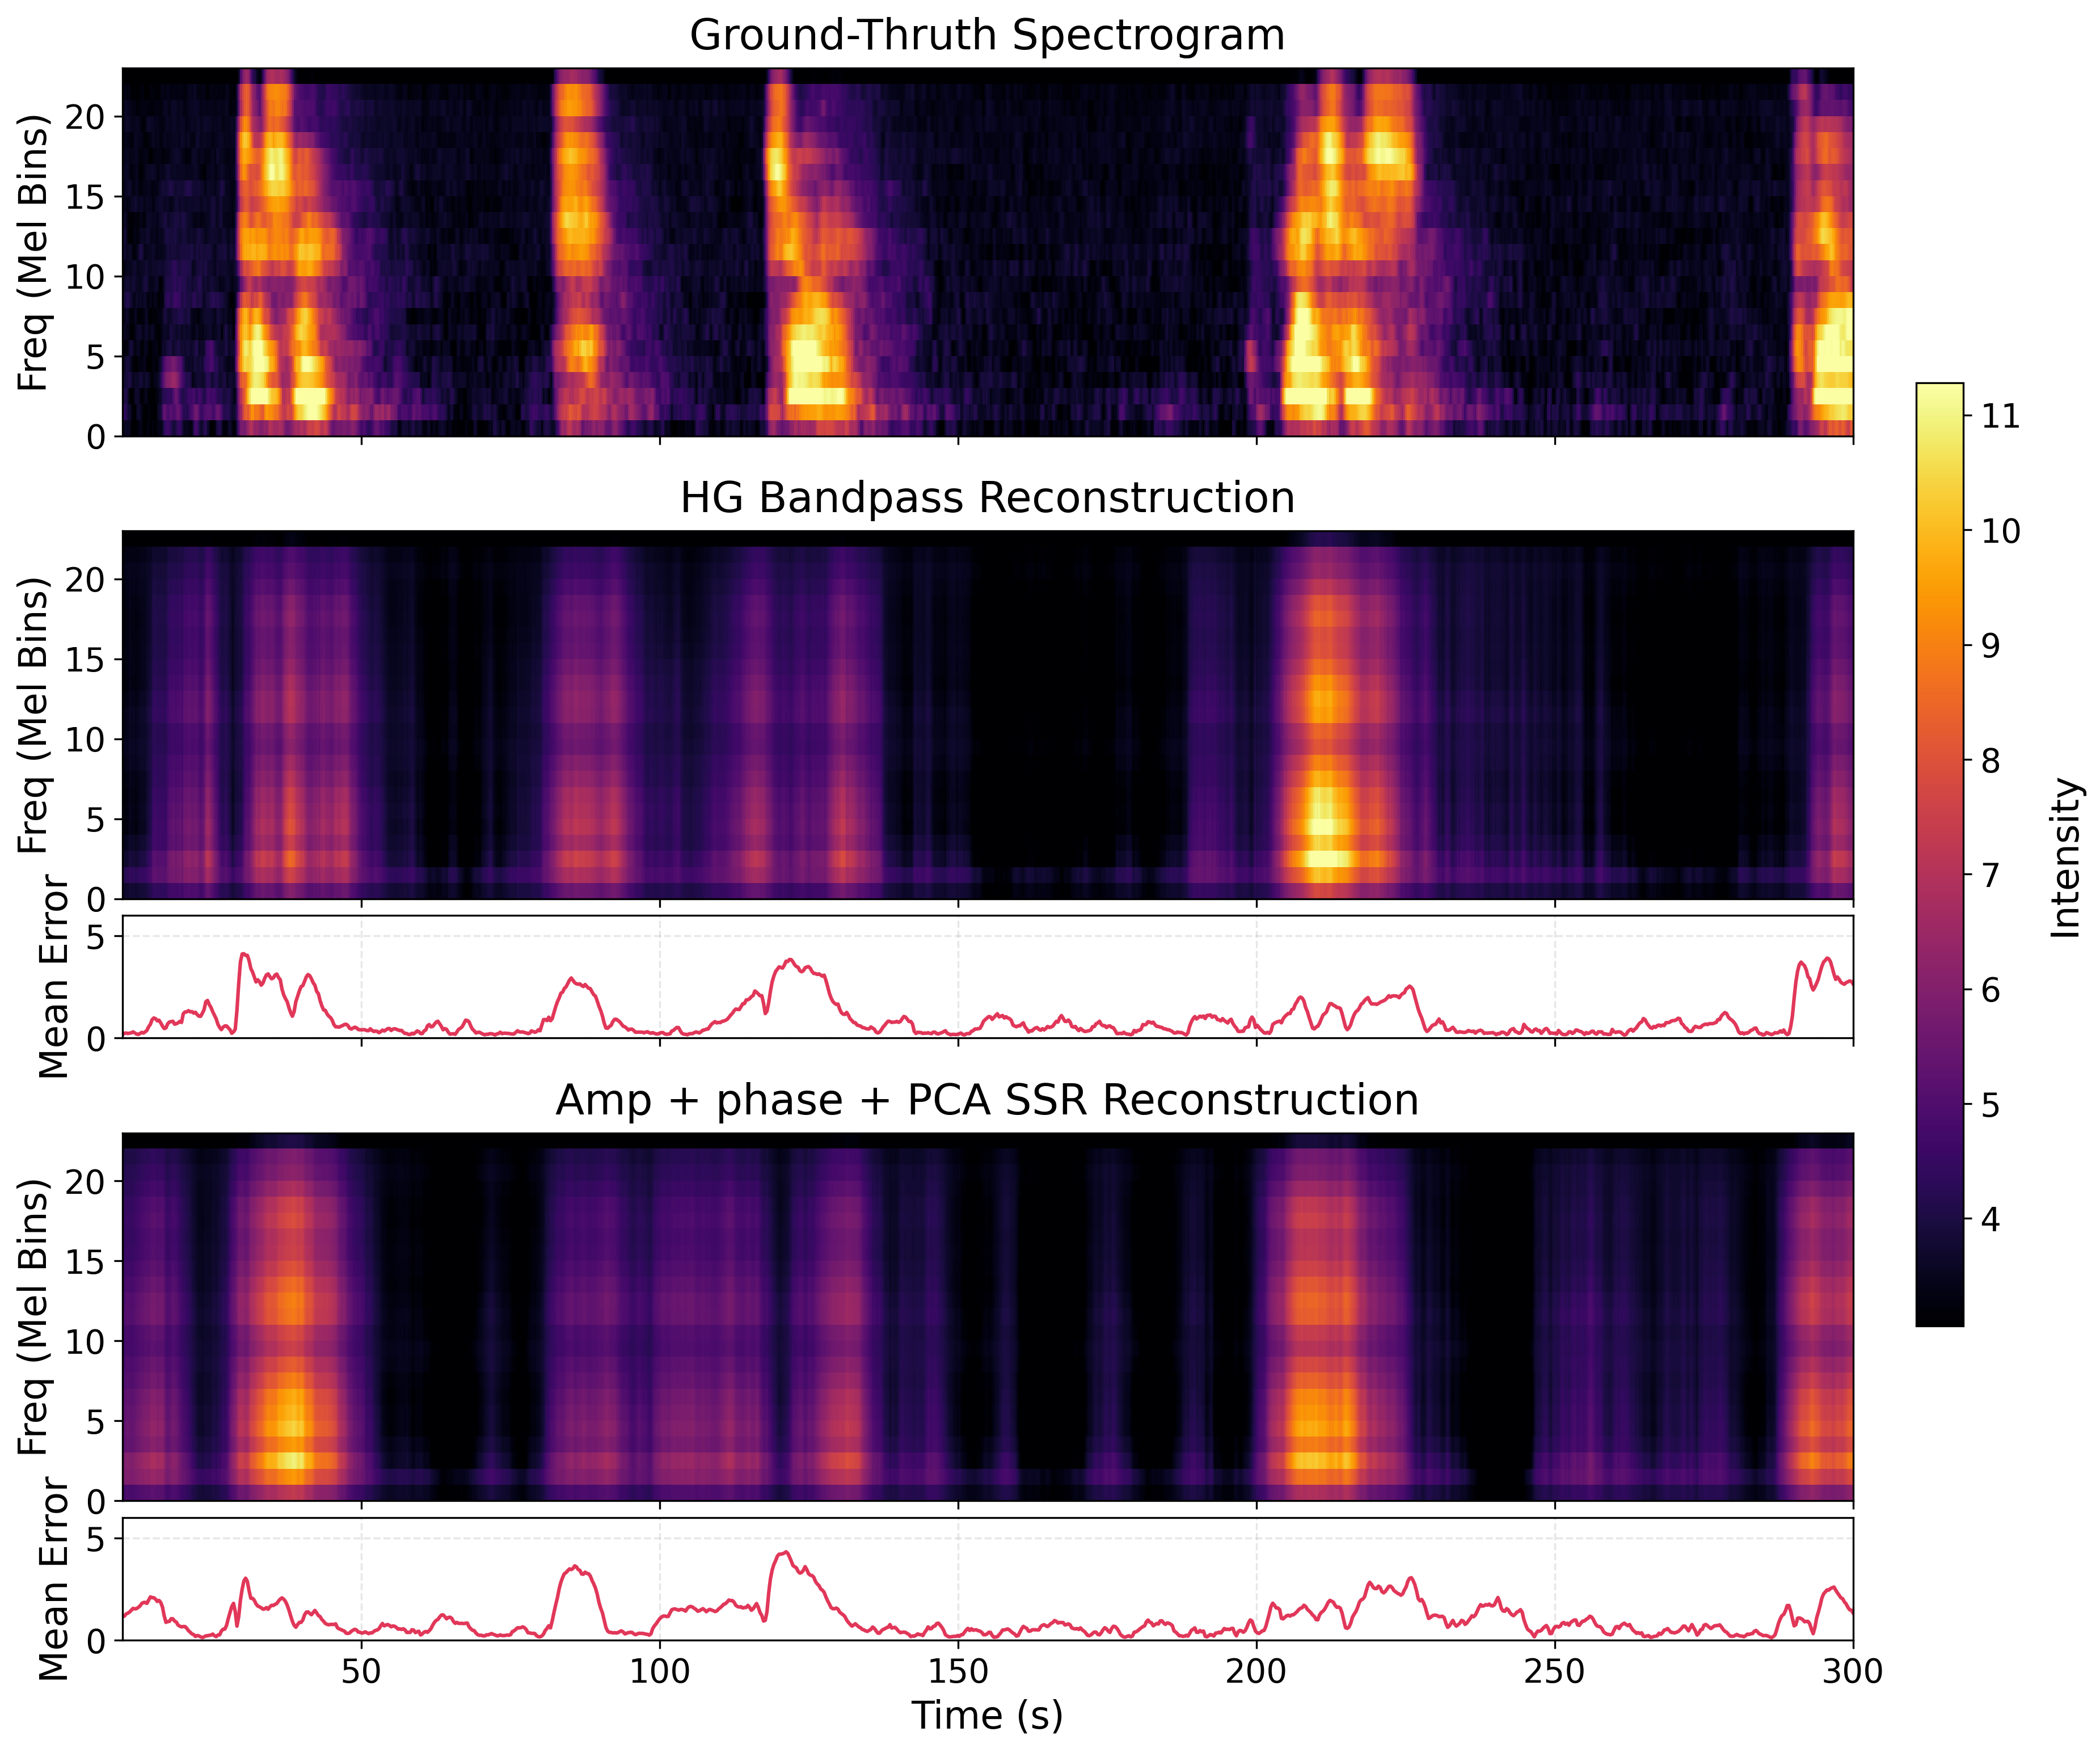
\includegraphics[width=0.70\textwidth]{images/zoomed_spectograms_sub1.png}
    \caption{Mel-spectrogram comparisons and absolute error tracks for a 10\,s excerpt of sub-01. The SSR model used amplitude, phase, and PAC features. Reconstructions for all participants are shown in appendix~\ref{app:spetrogramsrec}. \todo{the time axis of this figure is labelled 10--300\,s but shows a 10\,s excerpt; fix in report\_figures.ipynb (cell 11), also titles ``Ground-Thruth'' and ``PCA''}}
    \label{fig:spectrograms}
\end{figure}

\subsection{Feature extraction runtime}

Kalman filtering required an average of $1.44\text{ ms}$ per channel per $50\text{ ms}$ block (median: $1.39\text{ ms}$; 95th percentile of channel-mean times: $1.60\text{ ms}$), i.e.\ about 0.29\,ms per channel per 10\,ms frame. Deriving the complete multi-channel feature vector (amplitude, phase, and PAC features across all tracked oscillators) required an average of $5.37\text{ ms}$ per frame across participants (95th percentile: $6.83\text{ ms}$; 99th percentile: $7.42\text{ ms}$). Feature stacking across temporal context windows required $0.017\text{ ms}$ on average. For a participant with 127 channels, the per-sample Kalman filter thus needs about 9\,ms per 10\,ms frame even when spread over four threads, so that together with feature derivation the Python implementation does not yet meet the 10\,ms frame budget. The steady-state form of the filter removes this bottleneck: updating the states of all 127 channels of sub-01 (740 oscillators) sample by sample took 0.095\,ms per 10\,ms frame (95th percentile 0.117\,ms) in vectorized NumPy on a single core of a 2.1\,GHz Intel Xeon virtual machine, i.e.\ about 1\% of the frame budget (all participants: 0.05--0.13\,ms per frame, 95th percentiles 0.07--0.21\,ms), while the window statistics of the features are cheap running means.

\section{Discussion}

\subsection{Principal findings}

SSR features, extracted causally with oscillator parameters estimated once from 10\,s of data, reconstructed speech as accurately as causal bandpass features in a pipeline that had been designed around the latter. This held at every level of the feature hierarchy: amplitude alone, amplitude with low-frequency phase, and with PAC, with mean differences of at most 0.007 in correlation and 95\% confidence intervals that excluded differences larger than about 0.01--0.02. Low-frequency information improved reconstruction by about 0.02 in both frameworks, PAC added little, and both causal pipelines were slightly (0.004--0.011) below the offline bandpass pipeline that uses future samples.

We consider this parity the central result, because it was obtained on terms set by the bandpass approach: 50\,ms windows, a linear decoder tuned for envelopes, and a bandpass baseline that we made as strong as possible for a causal setting by applying the original zero-phase filters to a buffer of past data. The matched-bandpass comparison sharpens the interpretation. When the bandpass filters were placed at exactly the frequencies and bandwidths of the SSR oscillators, the two estimators gave practically identical decoding accuracy. The value of SSR in this pipeline therefore lies less in a better estimate of a given band than in what comes with the model: the frequencies are identified for each participant and channel from a few seconds of data rather than fixed in advance, every oscillator is a causal quadrature filter whose delay is a few milliseconds in the high-gamma range (section~\ref{sec:res_filters}), amplitude and phase are available at every sample without a buffer or Hilbert transform, and all of this costs about 0.1\,ms per 10\,ms frame for a full montage. Real-time estimation of low-frequency phase is otherwise only possible with windowed narrow-band filtering combined with forecasting of the signal~\cite{Zrenner2020,McIntosh2020}, whereas SSR provides it sample by sample~\cite{Wodeyar2021}. SSR thus offers a coherent framework for combining subject-specific high-gamma amplitude, low-frequency phase and cross-frequency features in a streaming decoder, at no cost in accuracy relative to the best causal bandpass features we could construct.

The results do not show that SSR phase is intrinsically more informative than bandpass phase: both frameworks gained similarly from low-frequency information. The low-frequency bandpass features also encode the slow voltage fluctuations themselves (the cosine of the Hilbert phase times the Hilbert amplitude is the low-passed signal), which are informative for movement and speech decoding~\cite{Schalk2007,Proix2022}. That low-frequency amplitude alone did not improve the bandpass features suggests that the useful information is in the timing of slow fluctuations rather than in their power. The small but consistent advantage of the offline pipeline shows that the remaining gap is due to causality rather than to the feature type: whole-recording zero-phase filtering and the Hilbert transform use future samples, and both causal estimators lose a similar amount by not doing so. An offline counterpart of SSR, the Kalman smoother, would be the corresponding non-causal reference for SSR features.

\subsection{Implications for feature extraction}

The oscillator-distribution and PLS-weight analyses suggest that informative neural activity was not confined to a single fixed spectral range across all participants. Some participants showed localized high-weight clusters, whereas others showed flatter weight profiles and weaker high-gamma/non-high-gamma separation. This is consistent with the clinical origin of the recordings: electrode locations were determined by seizure-monitoring needs, not by a speech-decoding sampling plan. Subject-specific oscillator tracking may therefore be particularly useful when electrode coverage and spectral profiles vary substantially across participants.

The stability analysis also suggests that oscillator parameters initialized from a short segment can remain useful over subsequent folds. This is encouraging for streaming applications, where continuous re-estimation may be undesirable. Because the decoder was retrained in every fold on data from both before and after the test segment, this analysis is, however, only an indirect test of parameter drift. A forward-chaining evaluation (training on early and testing on progressively later data) and comparison with periodically re-initialized parameters would test drift directly, and longer-duration online tests would be necessary before drawing conclusions about recalibration frequency or clinical deployment.

\subsection{Latency}

Two latencies should be distinguished. The feature latency of SSR is short: the group delay of the SSR high-gamma oscillators is a few milliseconds (median 6.2\,ms, at most 29\,ms) and that of most low-frequency oscillators tens of milliseconds (section~\ref{sec:res_filters}). A causal bandpass filter can have a similar delay (7.7\,ms at 120\,Hz for the fourth-order Butterworth filter), but the 409-tap FIR filters used in an earlier version of this analysis delayed their output by 199\,ms, and with a symmetric $\pm200$\,ms context such a delay shifts the neural window that the decoder sees for one feature type but not the other. Feature delays must therefore be matched or reported when feature types are compared; here we did so by using the same buffered zero-phase filters for all causal bandpass features. The decoder latency, in turn, is set by the temporal context: stacking 200\,ms of future windows, as in the original framework, implies 200\,ms of look-ahead for every feature set. With past-only context, which an online system requires, performance changed little (section~\ref{sec:res_decoding}): the high-gamma envelope alone did slightly better with past-only context, whereas the feature sets with low-frequency phase did slightly better with future context, possibly because slow responses that follow the acoustics, such as responses to the participant's own voice, carry information about the spectrogram.

The current Python implementation of the per-sample Kalman filter does not fit within the 10\,ms frame budget for the full montage (about 9\,ms per frame for 127 channels on four threads, plus 5.4\,ms for feature derivation). Because the parameters are fixed, however, the filter can be run in its steady-state form, which reduces each update to a few complex multiplications per oscillator and makes the computational cost negligible (section~\ref{sec:res_filters}). Feature derivation can likewise be made incremental by updating running window sums rather than recomputing each 50\,ms window.

\subsection{Limitations and future work}

Several limitations should constrain the interpretation of these results. First, the dataset consists of overt word reading in epilepsy participants. The clinical motivation is speech restoration for people with ALS, locked-in syndrome, or other severe motor-speech impairments, but attempted speech and silent speech can differ substantially from overt articulation. The present results should therefore be treated as evidence for overt-speech feature extraction, not as direct evidence for attempted-speech neuroprosthetic performance.

Second, the analysis uses a single public dataset with clinically determined electrode coverage. The number, location, and anatomical distribution of electrodes vary across participants and were not optimized for speech decoding. This limits generalizability and may explain part of the participant-level heterogeneity, including the decrease with low-frequency features in sub-09 and the participant-specific differences between amplitude-only SSR and the high-gamma envelope (from $-0.029$ to $+0.015$). Replication in additional cohorts and with more systematic speech-area coverage is required.

Third, parity is not superiority. The confidence intervals exclude differences larger than about 0.01--0.02 in correlation between SSR and causal bandpass features, but with ten participants smaller differences cannot be ruled out, and the gain from low-frequency information did not survive correction for multiple comparisons. The PAC features, as defined on 50\,ms windows, are largely redundant with high-gamma amplitude (section~\ref{sec:res_pac}), and neither they nor their phase-resolved variant improved reconstruction; cross-frequency features should therefore be considered exploratory in the present analysis. Richer decoders that can form nonlinear combinations of amplitude and phase may be needed to exploit them.

Fourth, the SSR parameter-initialization pipeline used heuristic safeguards, including the enforced minimum number of oscillators and the high-gamma fallback template, which supplied the high-gamma oscillators of 21\% of all channels and of 77\% of the channels in sub-06. These choices were motivated by the need to ensure high-gamma coverage across channels, but they should be replaced or validated with a more principled model-selection procedure. A small number of very slow oscillators also had damping parameters marginally above one; the steady-state filters were nevertheless stable for all channels.

Finally, the number of PLS components was selected by nested cross-validation over a grid of 4 to 12 components. The high-gamma-only feature sets chose the smallest value in half of the folds, so their accuracy may be slightly underestimated, and the decoder is linear. The comparison should be repeated with nonlinear decoders, longer recordings, and in online, closed-loop use.

\section{Conclusion}

SSR-derived oscillatory features supported overt-speech spectrogram reconstruction from sEEG as well as conventional bandpass features in a fully causal pipeline, at every level from amplitude alone to amplitude, low-frequency phase and PAC, and as well as bandpass filters placed at exactly the same frequencies. Low-frequency information improved reconstruction in both frameworks, and PAC added little. Because SSR achieves this parity while identifying subject-specific frequencies automatically and estimating amplitude and phase sample by sample, with millisecond delays and negligible computational cost, state-space oscillatory modelling is a promising feature-extraction strategy for real-time speech neuroprostheses. Stronger conclusions require replication across datasets, nonlinear decoders, and validation in attempted-speech and closed-loop settings.

\appendix

\section{Electrode locations in participants}
\label{app:electrode_locations}

Electrode locations were determined by clinical necessity, and between 54 and 127 contacts per participant were recorded. The majority of electrodes were located in white matter (40.3\%) or unlabeled regions (12.6\%). Unlabeled regions included contacts that could not be assigned to a cortical or subcortical label, for example because they were located just outside cortex. Other electrodes were predominantly located in the superior temporal sulcus, hippocampus, and inferior parietal gyrus (figure~\ref{fig:channelDistribution}).

\begin{figure}[!htb]
     \centering
    \begin{subfigure}[b]{0.95\textwidth}
         \centering
         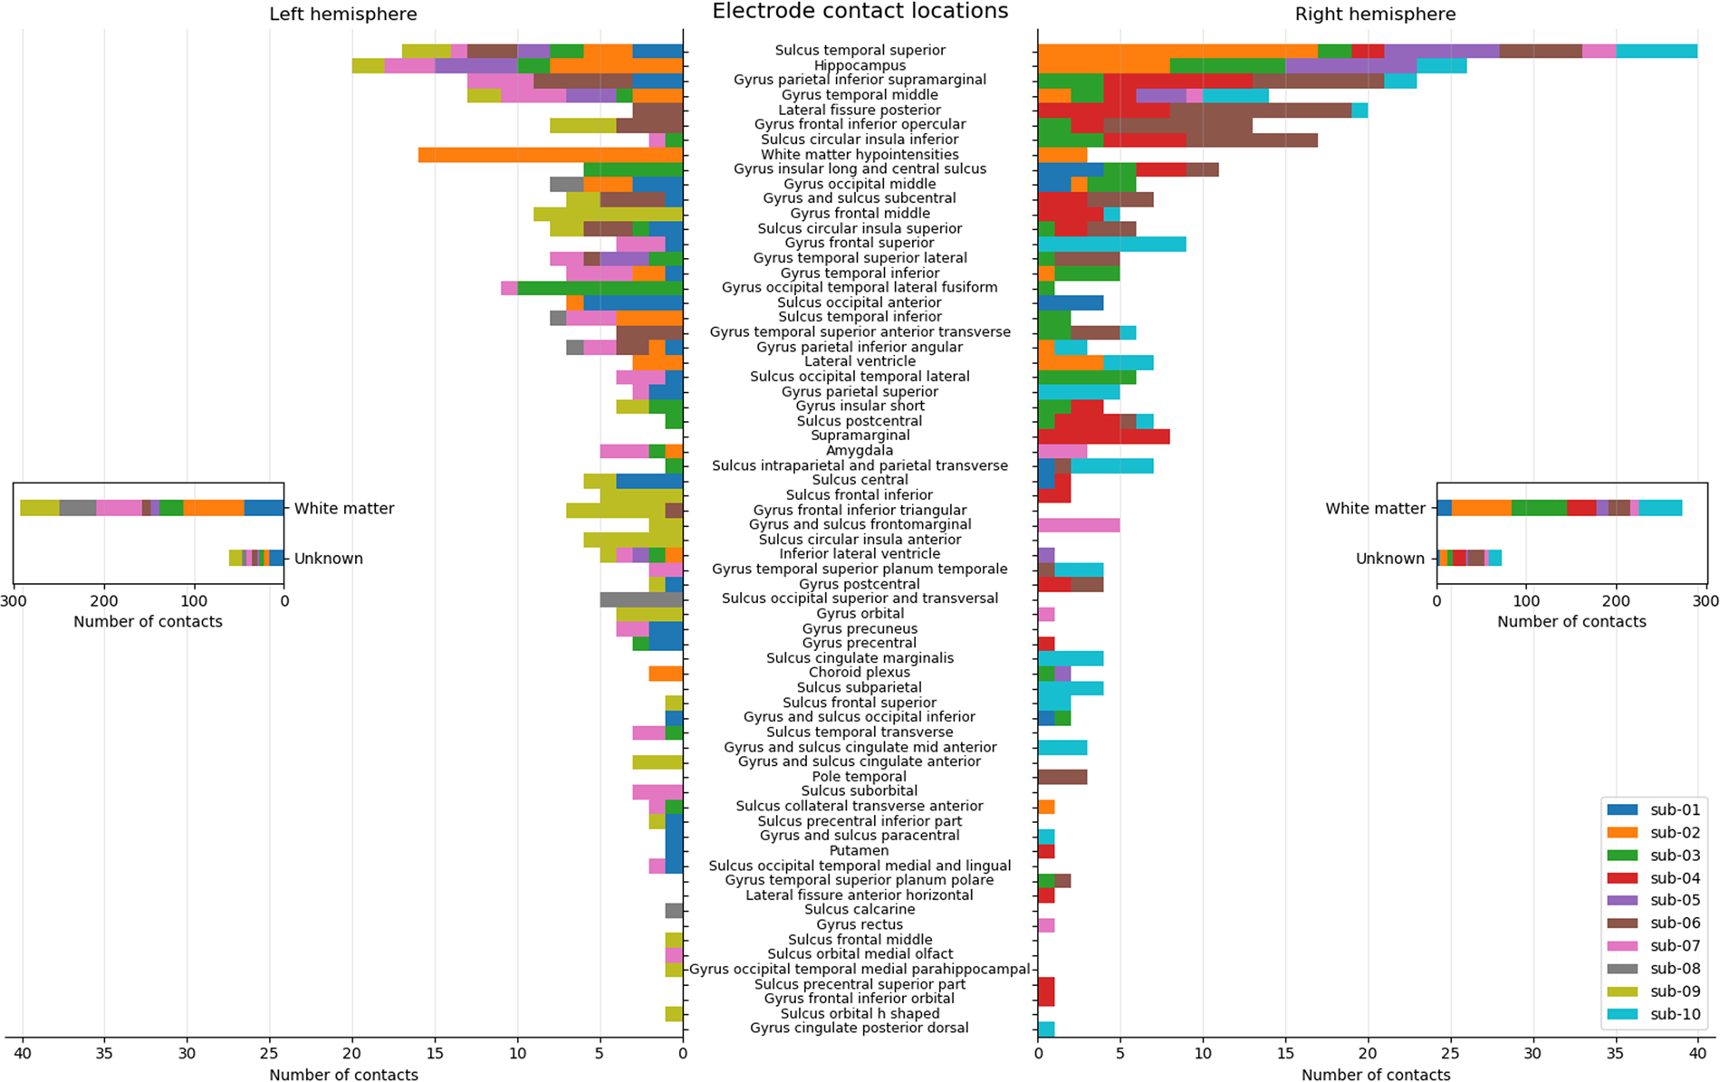
\includegraphics[width=\textwidth]{channel_region_distribution}
         \caption{Distribution by region.}
     \end{subfigure}

     \vspace{0.75em}

     \begin{subfigure}[b]{0.95\textwidth}
         \centering
         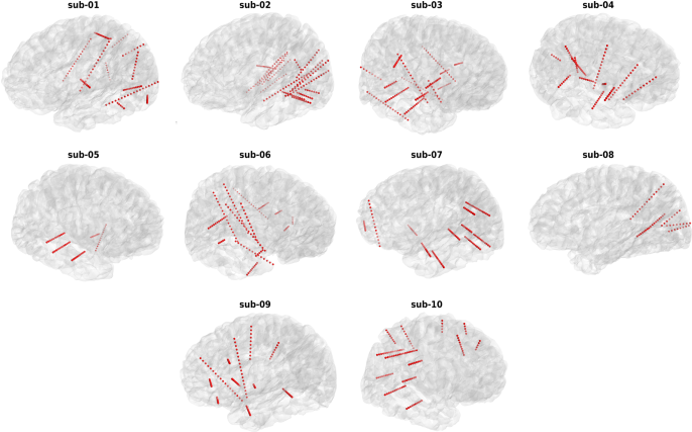
\includegraphics[width=\textwidth]{participant_ch_regions}
         \caption{Distribution by participant. Each red sphere represents an implanted electrode channel.}
     \end{subfigure}
     \caption{Electrode distribution across participants. Figure adapted from Verwoert et al.~\cite{dataset}.}
     \label{fig:channelDistribution}
\end{figure}

\section{Parameter initialization pipeline}
\label{app:algorithm}

Algorithm~\ref{alg:parameter_init} summarizes the parameter-initialization procedure used to obtain oscillator frequencies, damping coefficients, and process variances for each channel.

\begin{algorithm}[!htb]
\caption{Parameter initialization pipeline.}
\label{alg:parameter_init}
\begin{algorithmic}[1]
\REQUIRE First 10 seconds of raw iEEG channel data
\ENSURE Set of oscillator parameters for each channel: frequencies ($\omega$), damping coefficients ($a$), and process driving variances ($Q$)

\FORALL{subjects}
    \FORALL{channels}
        \STATE Run iterative SOMATA search algorithm up to 7 iterations
        \IF{optimal model has fewer than 3 oscillators}
            \STATE Select the 3-oscillator model
        \ENDIF
        \IF{optimal model contains a high-gamma oscillator (70--170 Hz)}
            \STATE Extract parameters ($\omega,a,Q$) from the optimal model
        \ELSE
            \STATE Search higher-iteration SOMATA models for high-gamma components
            \IF{high-gamma oscillator is found in a more complex model}
                \STATE Extract parameters from the simplest model containing a high-gamma component
            \ELSE
                \STATE Append participant-level high-gamma template frequencies and parameter averages from other channels
            \ENDIF
        \ENDIF
    \ENDFOR
\ENDFOR
\RETURN $\omega,a,Q$
\end{algorithmic}
\end{algorithm}

Figure~\ref{fig:freq_cluster} shows the participant-level frequency templates used when the fallback step was required. For sub-01, sub-02, sub-03, sub-04, sub-08, and sub-10, extracted high-gamma peaks clustered between 70 and 90 Hz. Sub-05 and sub-09 had both peaks above 100 Hz, and sub-06 and sub-07 had one peak between 70 and 90 Hz and another above 100 Hz. The template was added to 50 (sub-01), 62 (sub-02), 17 (sub-03), 45 (sub-04), 7 (sub-05), 114 (sub-06), 7 (sub-07), 15 (sub-08), 60 (sub-09) and 51 (sub-10) channels.

\begin{figure}[!htb]
    \centering
    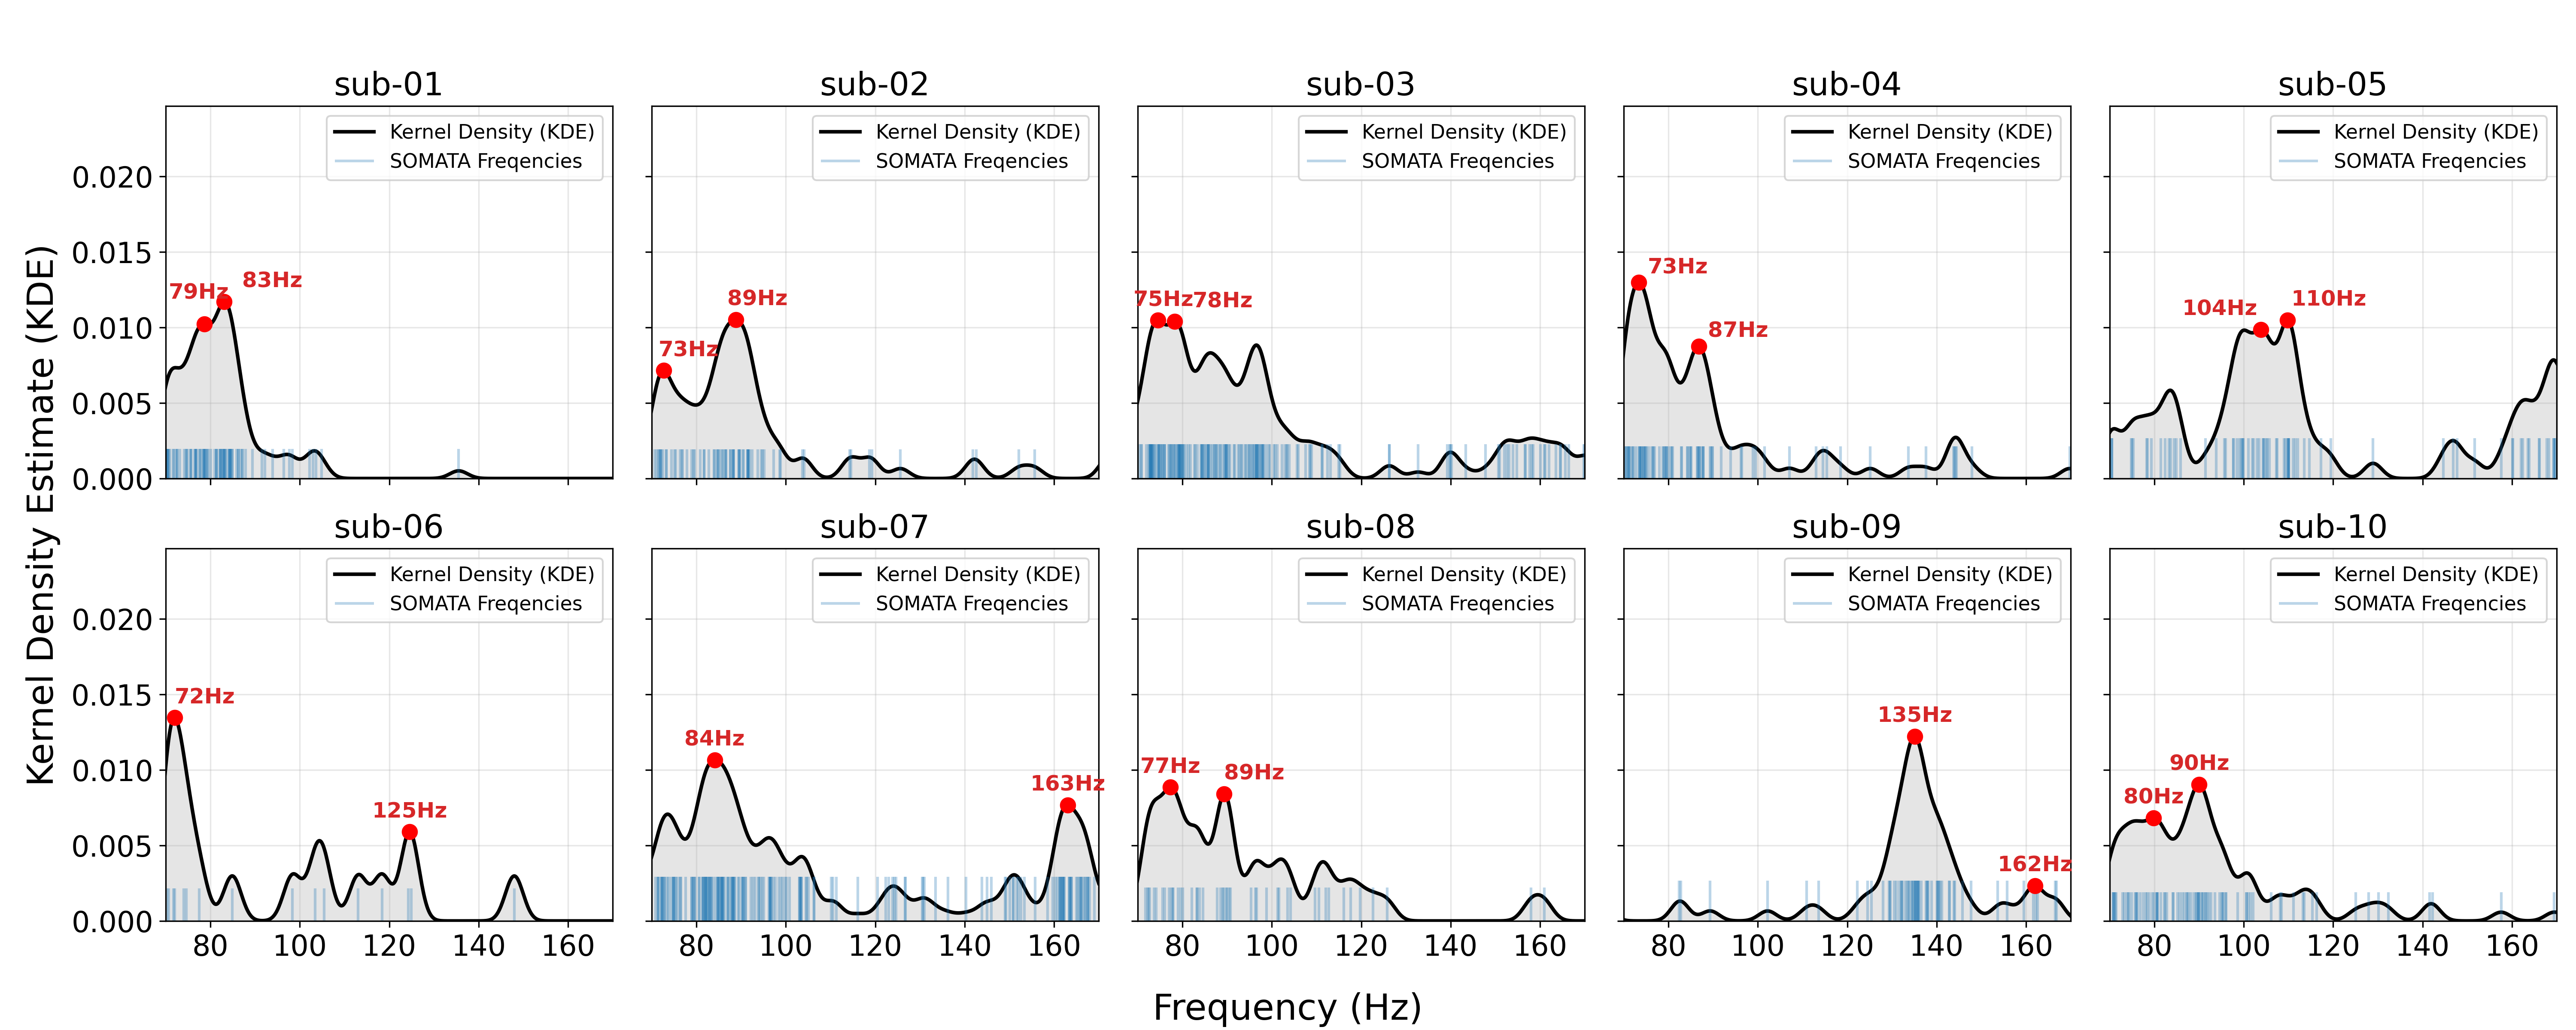
\includegraphics[width=\linewidth]{images/SOMATA_density_templates_all_subjects.png}
    \caption{Participant-level high-gamma frequency templates. Blue vertical lines indicate high-gamma frequencies found across channels. A Gaussian KDE smooths the distribution, and final template frequencies are selected with SciPy's \texttt{find\_peaks} algorithm.}
    \label{fig:freq_cluster}
\end{figure}

\section{PLS hyperparameter optimization}
\label{app:PLS_n_components}

The number of PLS components was selected separately for each of the five models. HG bandpass features reached their highest validation performance at six components, HG with Low-Pass features reached their highest validation performance at nine components. All SSR feature sets performed best with eight components (figure~\ref{fig:opt_n_components}). Between 6 and 11 components, mean performance varied by less than 0.01 for every model; with fewer components, performance dropped most for the larger feature sets (e.g.\ HG + LP: $r=0.749$ with five and $r=0.719$ with three components).

\begin{figure}[!htb]
    \centering
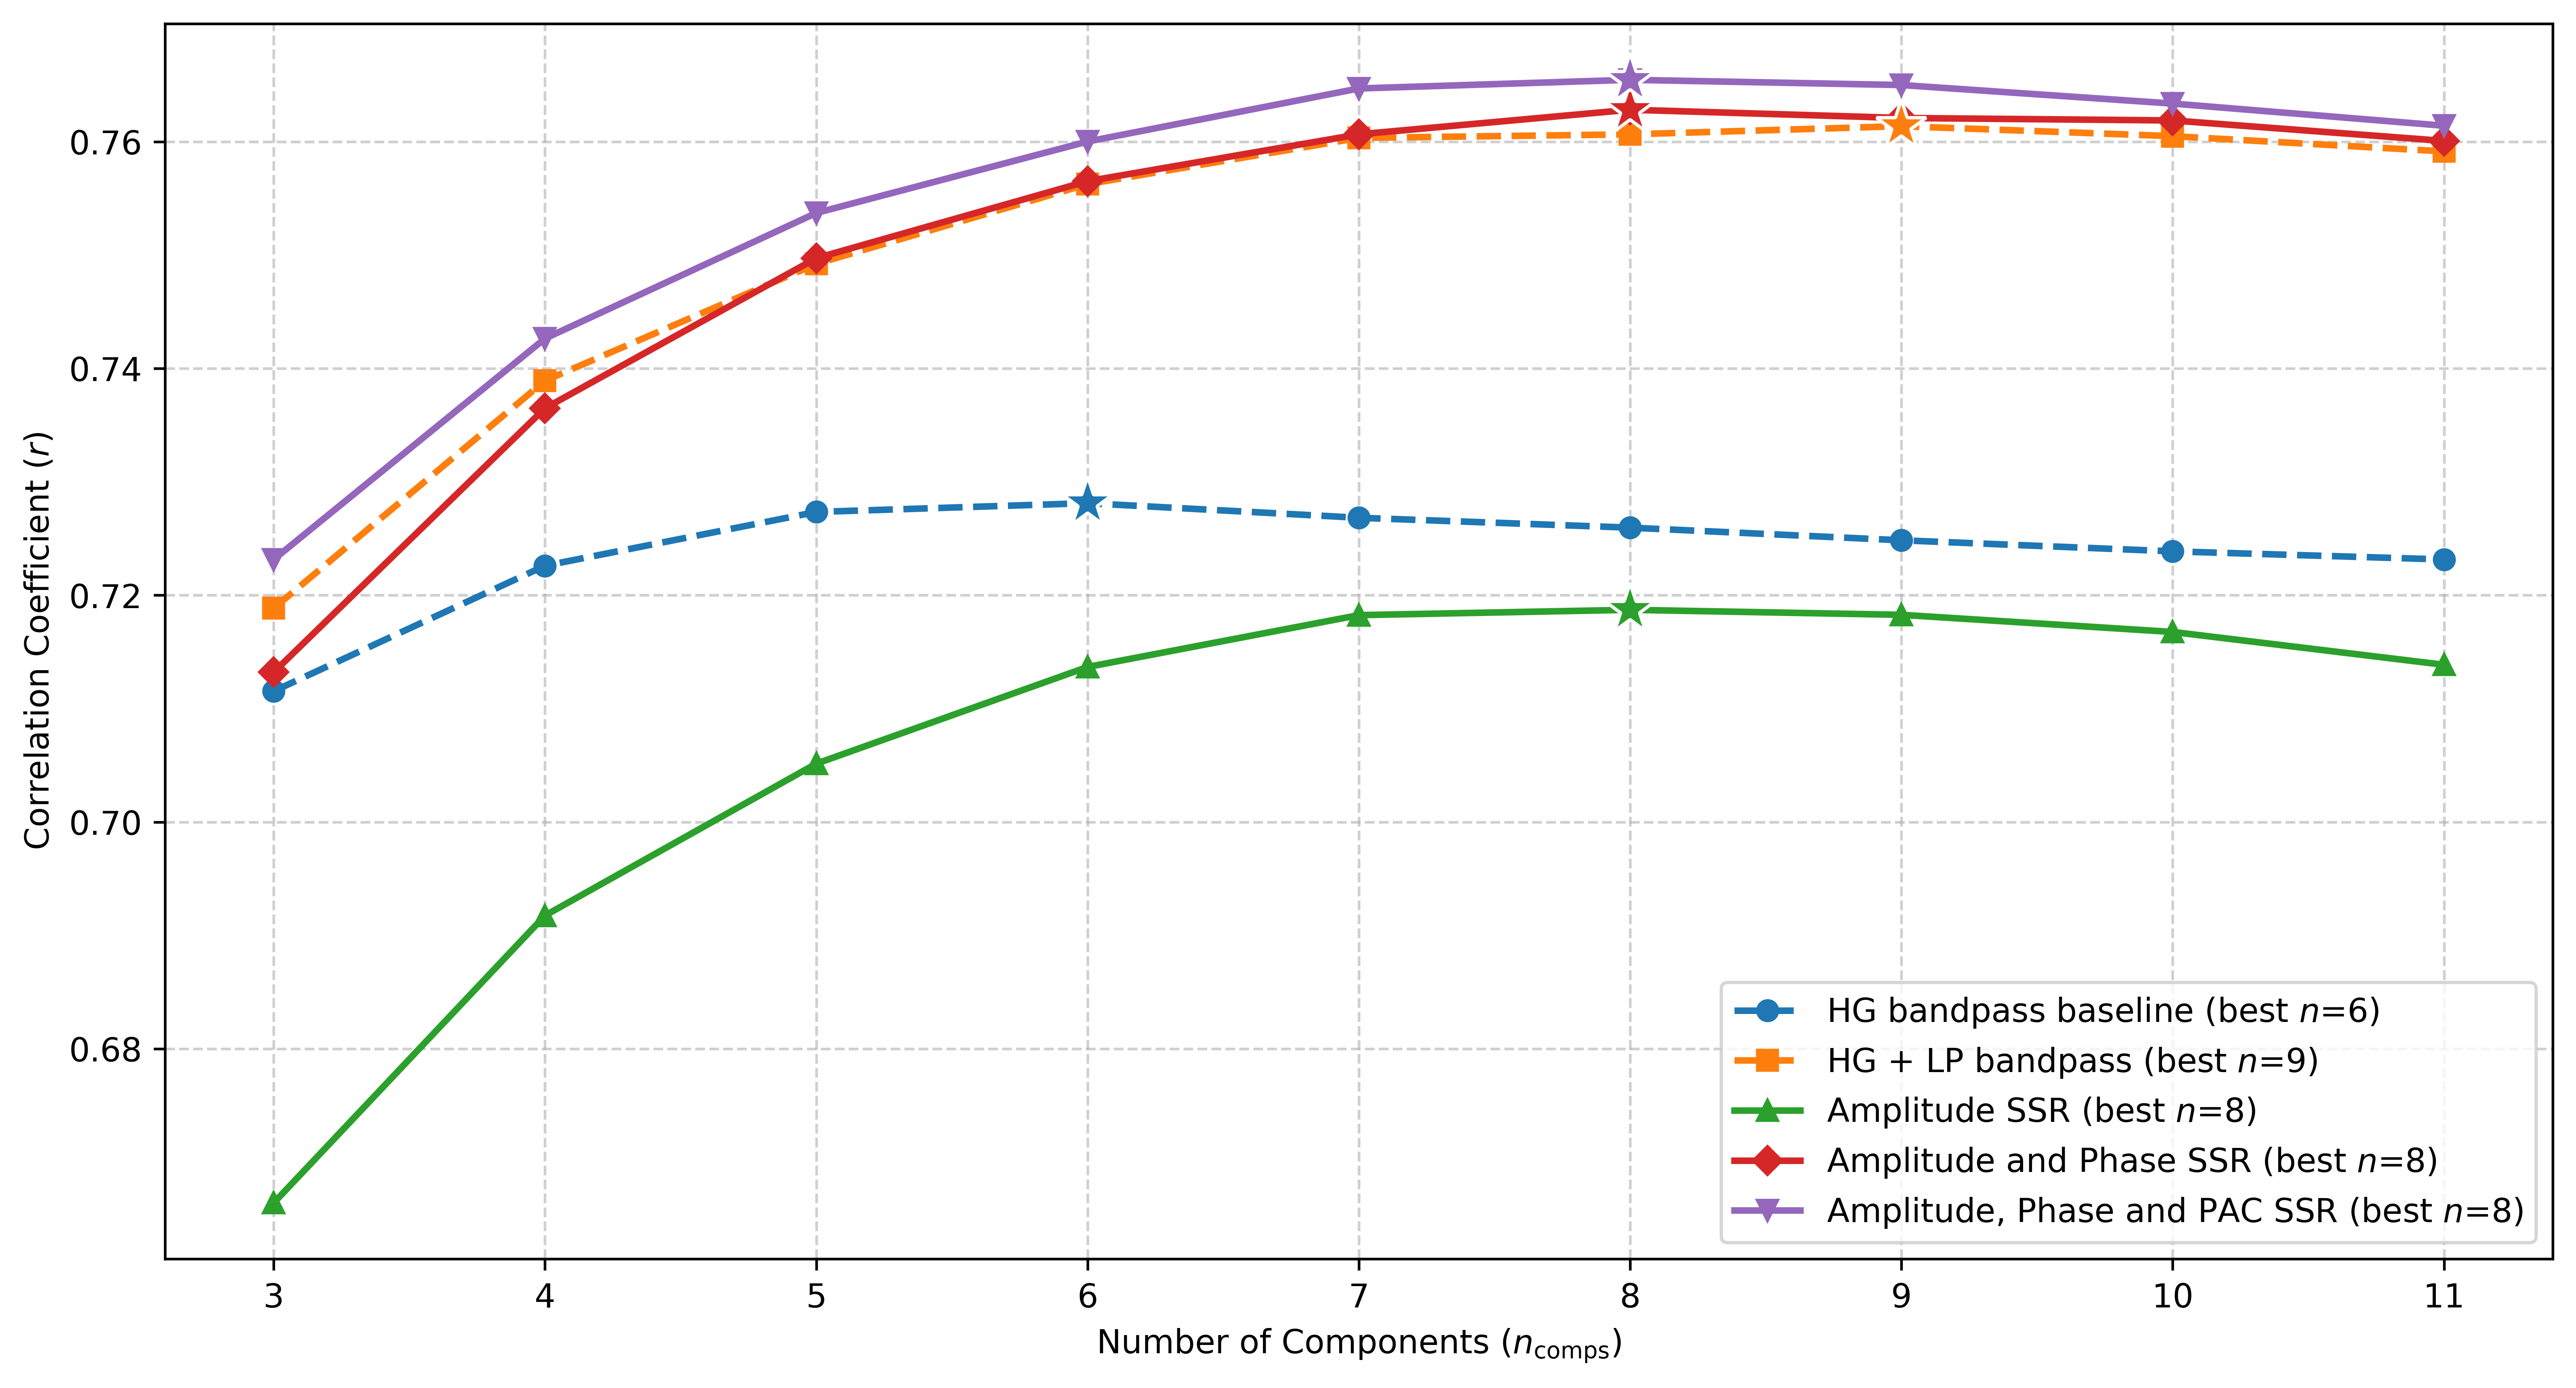
\includegraphics[width=\linewidth]{images/hyperparameter.png}
    \caption{Hyperparameter search for the optimal number of components in the PLS decoder for different feature sets.}
    \label{fig:opt_n_components}
\end{figure}

\section{Temporal stability}
\label{app:tempstability}

SSR performance remained stable across consecutive validation folds (figure~\ref{fig:fold_stability}). The trend lines suggest that the gap between SSR and the bandpass baseline was not driven by a single late or early segment, and the bandpass baseline showed a similar small downward trend, indicating that the trend reflects the data rather than degradation of the SSR parameters. Because SSR parameters were initialized from the first 10 seconds only, this stability indicates that the fitted oscillator parameters remained useful over the later segments of the recording, although longer recordings and online validation would be needed to assess parameter drift more rigorously.

\begin{figure}[!htb]
    \centering
    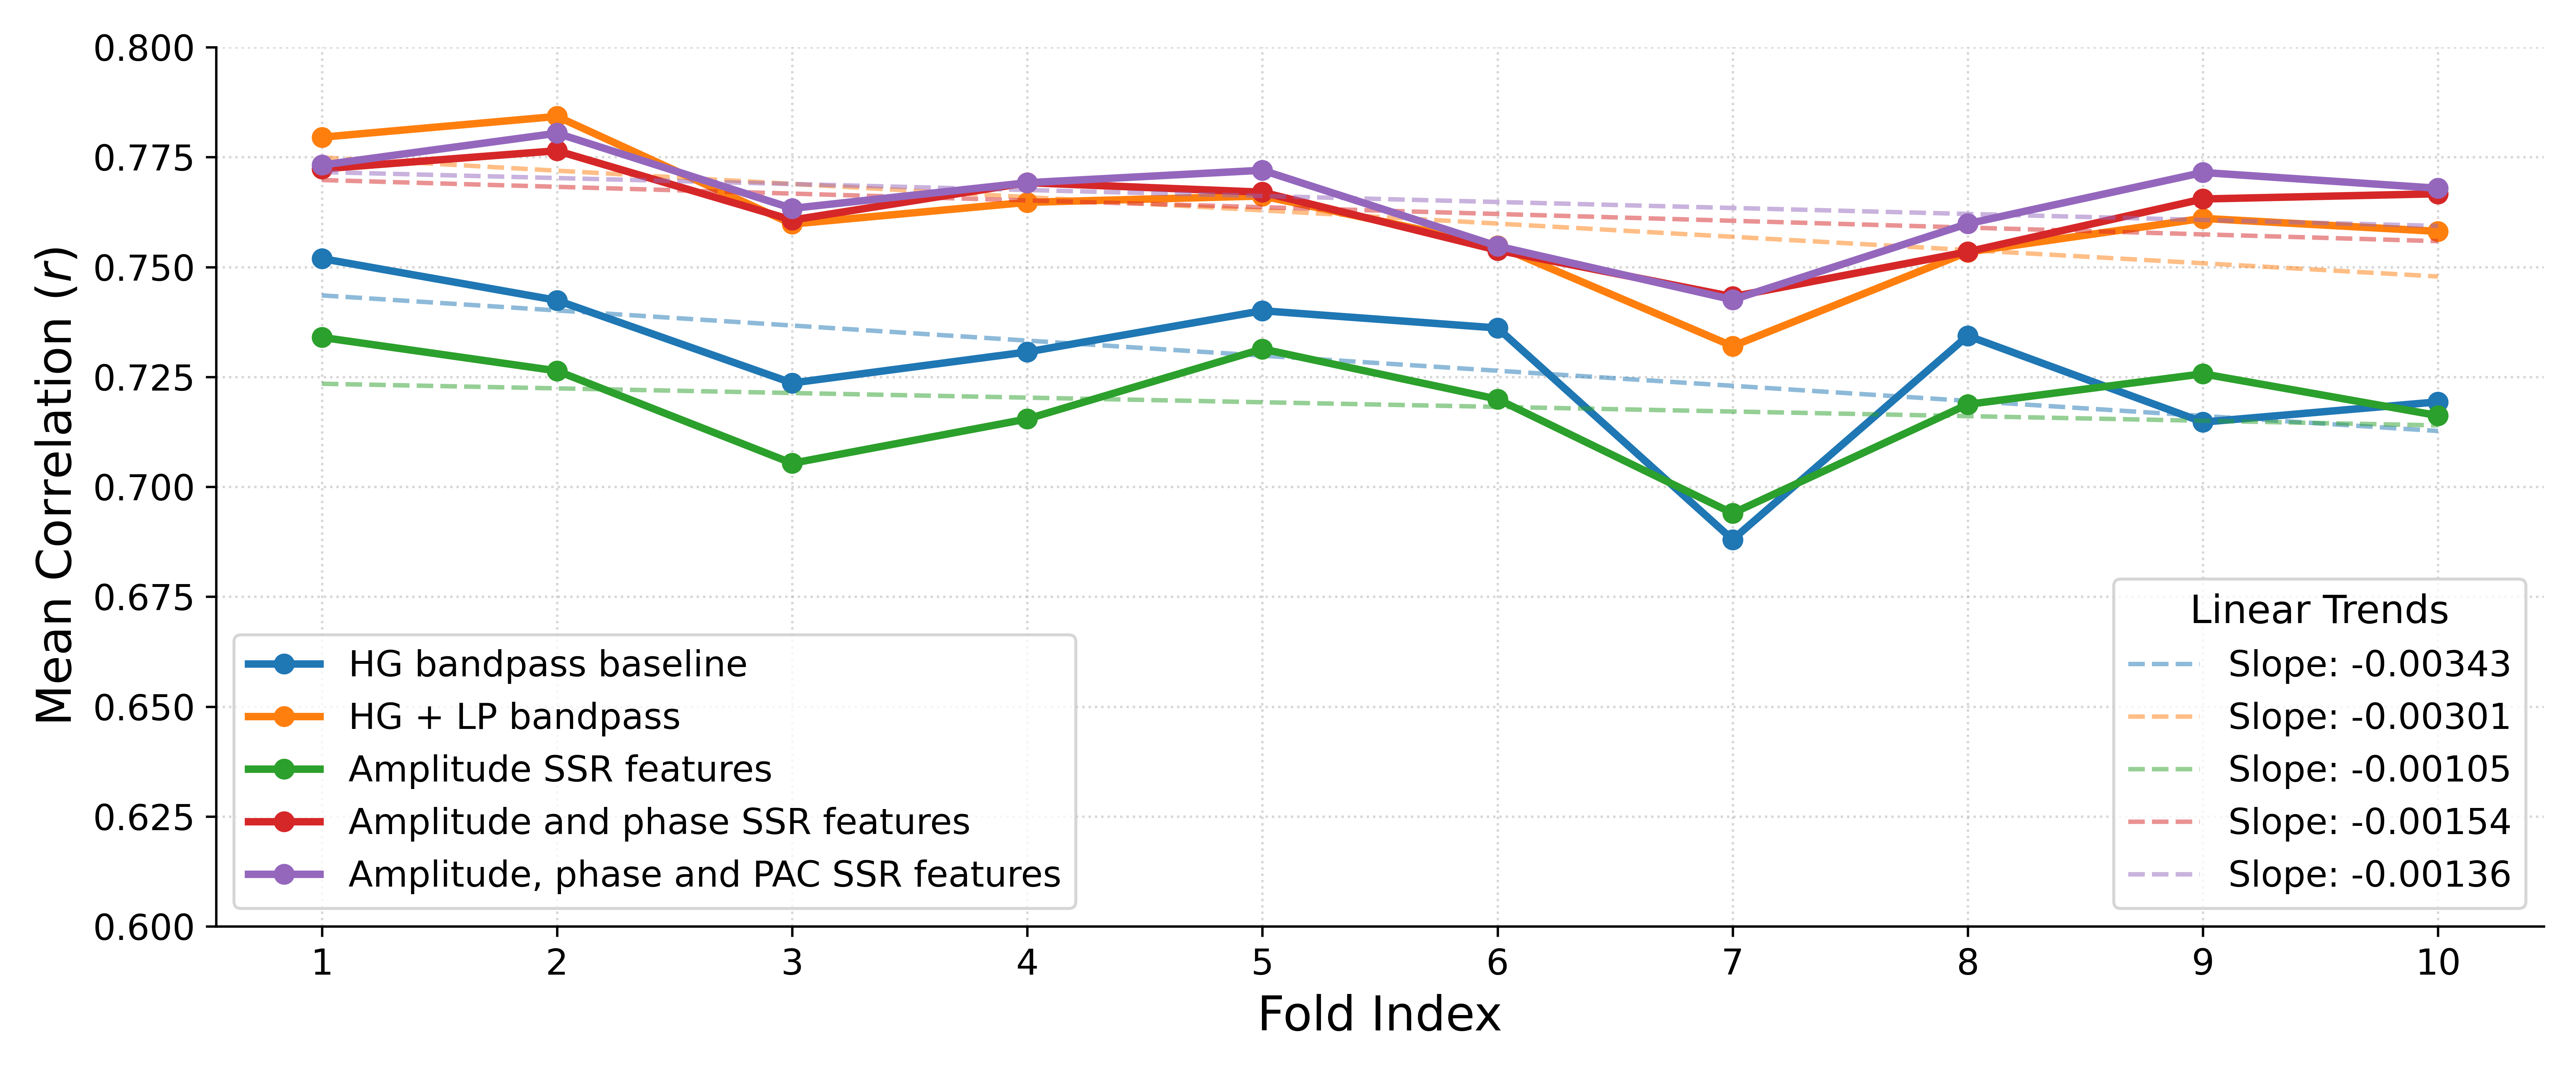
\includegraphics[width=0.80\linewidth]{images/fold_stability_trends_new.png}
    \caption{Performance stability across validation folds. Each fold represents a consecutive segment of approximately 29\,s, with dashed lines indicating linear trends and their slopes.}
    \label{fig:fold_stability}
\end{figure}


\section{Reconstructed spectrograms}
\label{app:spetrogramsrec}

\begin{figure}[!htb]
     \centering
     \begin{subfigure}[b]{0.48\textwidth}
         \centering
         \figorplaceholder[width=\textwidth]{images/sub-01_spectograms_vertical.png}
         \caption{Sub-01}
     \end{subfigure}
     \hfill
     \begin{subfigure}[b]{0.48\textwidth}
         \centering
         \figorplaceholder[width=\textwidth]{images/sub-02_spectograms_vertical.png}
         \caption{Sub-02}
     \end{subfigure}
     \hfill
     \begin{subfigure}[b]{0.48\textwidth}
         \centering
         \figorplaceholder[width=\textwidth]{images/sub-03_spectograms_vertical.png}
         \caption{Sub-03}
     \end{subfigure}
     \hfill
     \begin{subfigure}[b]{0.48\textwidth}
         \centering
         \figorplaceholder[width=\textwidth]{images/sub-04_spectograms_vertical.png}
         \caption{Sub-04}
     \end{subfigure}
    \caption{Reconstructed Mel-spectrogram comparisons for sub-01 to sub-04, showing ground-truth audio, bandpass reconstruction, and full SSR reconstruction.}
    \label{fig:spectrograms_part1}
\end{figure}

\begin{figure}[p]
     \centering
     \begin{subfigure}[b]{0.48\textwidth}
         \centering
         \figorplaceholder[width=\textwidth]{images/sub-05_spectograms_vertical.png}
         \caption{Sub-05}
     \end{subfigure}
     \hfill
     \begin{subfigure}[b]{0.48\textwidth}
         \centering
         \figorplaceholder[width=\textwidth]{images/sub-06_spectograms_vertical.png}
         \caption{Sub-06}
     \end{subfigure}
     \hfill
     \begin{subfigure}[b]{0.48\textwidth}
         \centering
         \figorplaceholder[width=\textwidth]{images/sub-07_spectograms_vertical.png}
         \caption{Sub-07}
     \end{subfigure}
     \hfill
     \begin{subfigure}[b]{0.48\textwidth}
         \centering
         \figorplaceholder[width=\textwidth]{images/sub-08_spectograms_vertical.png}
         \caption{Sub-08}
     \end{subfigure}
     \hfill
     \begin{subfigure}[b]{0.48\textwidth}
         \centering
         \figorplaceholder[width=\textwidth]{images/sub-09_spectograms_vertical.png}
         \caption{Sub-09}
     \end{subfigure}
     \hfill
     \begin{subfigure}[b]{0.48\textwidth}
         \centering
         \figorplaceholder[width=\textwidth]{images/sub-10_spectograms_vertical.png}
         \caption{Sub-10}
     \end{subfigure}
     \caption{Mel-spectrogram comparisons and absolute error tracks for sub-05 to sub-10. The SSR model used amplitude, phase, and PAC features.}
     \label{fig:spectrograms_allpts}
\end{figure}

\ack{The authors thank the creators of the public Verwoert et al. dataset and associated baseline codebase. TODO: add any additional acknowledgements required by the journal or institution.}

\funding{TODO: add funder names and grant numbers, or state that no specific funding was received.}

\roles{TODO: replace with confirmed CRediT contributor roles for all authors. Draft roles: Lisa Ponsteen: Conceptualization, Methodology, Software, Formal analysis, Visualization, Writing -- original draft. R. Cavill: Supervision, Methodology, Writing -- review and editing. C. Herff: Supervision, Methodology, Writing -- review and editing. A. Wodeyar: Supervision, Methodology, Writing -- review and editing.}

\data{The iEEG, audio, and stimulus-timing data used in this study are publicly available from Verwoert et al.~\cite{dataset}. The conventional baseline pipeline was adapted from the Verwoert et al. codebase. The SSR feature-extraction and analysis code is available at \url{https://github.com/wodeyara/SSR-neural-speech-decoding} \todo{add a release tag / persistent identifier (e.g.\ Zenodo DOI) before submission}.}

\bibliographystyle{iopart-num}
\bibliography{references}

\end{document}
